% !TeX encoding = UTF-8
% !TeX program = xelatex
% !TeX spellcheck = en_US

\documentclass[degree=bachelor]{thuthesis}
  % 学位 degree:
  %   doctor | master | bachelor | postdoc
  % 学位类型 degree-type:
  %   academic(默认)| professional
  % 语言 language
  %   chinese(默认)| english
  % 字体库 fontset
  %   windows | mac | fandol | ubuntu
  % 建议终版使用 Windows 平台的字体编译


% 论文基本配置,加载宏包等全局配置
% !TeX root = ./thuthesis-example.tex

% 论文基本信息配置

\thusetup{
  %******************************
  % 注意:
  %   1. 配置里面不要出现空行
  %   2. 不需要的配置信息可以删除
  %   3. 建议先阅读文档中所有关于选项的说明
  %******************************
  %
  % 输出格式
  %   选择打印版(print)或用于提交的电子版(electronic),前者会插入空白页以便直接双面打印
  %
  output = print,
  % 格式类型
  %   默认为论文(thesis),也可以设置为开题报告(proposal)
  % thesis-type = proposal,
  %
  % 标题
  %   可使用“\\”命令手动控制换行
  %
  title  = {清华大学学位论文 \LaTeX{} 模板\\使用示例文档 v\version},
  title* = {An Introduction to \LaTeX{} Thesis Template of Tsinghua
            University v\version},
  %
  % 学科门类
  %   1. 学术型
  %      - 中文
  %        需注明所属的学科门类,例如:
  %        哲学、经济学、法学、教育学、文学、历史学、理学、工学、农学、医学、
  %        军事学、管理学、艺术学
  %      - 英文
  %        博士:Doctor of Philosophy
  %        硕士:
  %          哲学、文学、历史学、法学、教育学、艺术学门类,公共管理学科
  %          填写“Master of Arts“,其它填写“Master of Science”
  %   2. 专业型
  %      直接填写专业学位的名称,例如:
  %      教育博士、工程硕士等
  %      Doctor of Education, Master of Engineering
  %   3. 本科生不需要填写
  %
  degree-category  = {工学硕士},
  degree-category* = {Master of Science},
  %
  % 培养单位
  %   填写所属院系的全名
  %
  department = {计算机科学与技术系},
  %
  % 学科
  %   1. 研究生学术型学位,获得一级学科授权的学科填写一级学科名称,其他填写二级学科名称
  %   2. 本科生填写专业名称,第二学位论文需标注“(第二学位)”
  %
  discipline  = {计算机科学与技术},
  discipline* = {Computer Science and Technology},
  %
  % 专业领域
  %   1. 设置专业领域的专业学位类别,填写相应专业领域名称
  %   2. 2019 级及之前工程硕士学位论文,在 `engineering-field` 填写相应工程领域名称
  %   3. 其他专业学位类别的学位论文无需此信息
  %
  % professional-field  = {计算机技术},
  % professional-field* = {Computer Technology},
  %
  % 姓名
  %
  author  = {薛瑞尼},
  author* = {Xue Ruini},
  %
  % 指导教师
  %   中文姓名和职称之间以英文逗号“,”分开,下同
  %
  supervisor  = {郑纬民, 教授},
  supervisor* = {Professor Zheng Weimin},
  %
  % 副指导教师
  %
  associate-supervisor  = {陈文光, 教授},
  associate-supervisor* = {Professor Chen Wenguang},
  %
  % 联合指导教师
  %
  % co-supervisor  = {某某某, 教授},
  % co-supervisor* = {Professor Mou Moumou},
  %
  % 日期
  %   使用 ISO 格式;默认为当前时间
  %
  % date = {2019-07-07},
  %
  % 是否在中文封面后的空白页生成书脊(默认 false)
  %
  include-spine = false,
  %
  % 密级和年限
  %   秘密, 机密, 绝密
  %
  % secret-level = {秘密},
  % secret-year  = {10},
  %
  % 博士后专有部分
  %
  % clc                = {分类号},
  % udc                = {UDC},
  % id                 = {编号},
  % discipline-level-1 = {计算机科学与技术},  % 流动站(一级学科)名称
  % discipline-level-2 = {系统结构},          % 专业(二级学科)名称
  % start-date         = {2011-07-01},        % 研究工作起始时间
}

% 载入所需的宏包

% 定理类环境宏包
\usepackage{amsthm}
% 也可以使用 ntheorem
% \usepackage[amsmath,thmmarks,hyperref]{ntheorem}

\thusetup{
  %
  % 数学字体
  % math-style = GB,  % GB | ISO | TeX
  math-font  = xits,  % stix | xits | libertinus
}

% 可以使用 nomencl 生成符号和缩略语说明
% \usepackage{nomencl}
% \makenomenclature

% 表格加脚注
\usepackage{threeparttable}

% 表格中支持跨行
\usepackage{multirow}

% 固定宽度的表格。
% \usepackage{tabularx}

% 跨页表格
\usepackage{longtable}

% 算法
\usepackage{algorithm}
\usepackage{algorithmic}

% 量和单位
\usepackage{siunitx}

% 参考文献使用 BibTeX + natbib 宏包
% 顺序编码制
\usepackage[sort]{natbib}
\bibliographystyle{thuthesis-numeric}

% 著者-出版年制
% \usepackage{natbib}
% \bibliographystyle{thuthesis-author-year}

% 生命科学学院要求使用 Cell 参考文献格式(2023 年以前的 author-date 格式)
% \usepackage{natbib}
% \bibliographystyle{cell}

% 本科生参考文献的著录格式
% \usepackage[sort]{natbib}
% \bibliographystyle{thuthesis-bachelor}

% 参考文献使用 BibLaTeX 宏包
% \usepackage[style=thuthesis-numeric]{biblatex}
% \usepackage[style=thuthesis-author-year]{biblatex}
% \usepackage[style=gb7714-2015]{biblatex}
% \usepackage[style=apa]{biblatex}
% \usepackage[style=mla-new]{biblatex}
% 声明 BibLaTeX 的数据库
% \addbibresource{ref/refs.bib}

% 定义所有的图片文件在 figures 子目录下
\graphicspath{{figures/}}

% 数学命令
\makeatletter
\newcommand\dif{%  % 微分符号
  \mathop{}\!%
  \ifthu@math@style@TeX
    d%
  \else
    \mathrm{d}%
  \fi
}
\makeatother

% hyperref 宏包在最后调用
\usepackage{hyperref}



\begin{document}

% 封面
\maketitle

% 学位论文指导小组、公开评阅人和答辩委员会名单
% 本科生不需要
% % !TeX root = ../thuthesis-example.tex

\begin{committee}[name={学位论文指导小组、公开评阅人和答辩委员会名单}]

  \newcolumntype{C}[1]{@{}>{\centering\arraybackslash}p{#1}}

  \section*{指导小组名单}

  \begin{center}
    \begin{tabular}{C{3cm}C{3cm}C{9cm}@{}}
      李XX & 教授     & 清华大学 \\
      王XX & 副教授   & 清华大学 \\
      张XX & 助理教授 & 清华大学 \\
    \end{tabular}
  \end{center}


  \section*{公开评阅人名单}

  \begin{center}
    \begin{tabular}{C{3cm}C{3cm}C{9cm}@{}}
      刘XX & 教授   & 清华大学                    \\
      陈XX & 副教授 & XXXX大学                    \\
      杨XX & 研究员 & 中国XXXX科学院XXXXXXX研究所 \\
    \end{tabular}
  \end{center}


  \section*{答辩委员会名单}

  \begin{center}
    \begin{tabular}{C{2.75cm}C{2.98cm}C{4.63cm}C{4.63cm}@{}}
      主席 & 赵XX                  & 教授                    & 清华大学       \\
      委员 & 刘XX                  & 教授                    & 清华大学       \\
          & \multirow{2}{*}{杨XX} & \multirow{2}{*}{研究员} & 中国XXXX科学院 \\
          &                       &                         & XXXXXXX研究所  \\
          & 黄XX                  & 教授                    & XXXX大学       \\
          & 周XX                  & 副教授                  & XXXX大学       \\
      秘书 & 吴XX                  & 助理研究员              & 清华大学       \\
    \end{tabular}
  \end{center}

\end{committee}



% 也可以导入 Word 版转的 PDF 文件
% \begin{committee}[file=figures/committee.pdf]
% \end{committee}


% 使用授权的说明
% 本科生开题报告不需要
\copyrightpage
% 将签字扫描后授权文件 scan-copyright.pdf 替换原始页面
% \copyrightpage[file=scan-copyright.pdf]

\frontmatter
% !TeX root = ../thuthesis-example.tex

% 中英文摘要和关键字

\begin{abstract}
  中微子实验依赖 PMT 捕获物理事例产生的少量光子,来对事例进行位置与时间重建,因此 PMT 的增益刻度对提高探测器的能量分辨率具有重要意义。
  包括 JUNO 在内的部分中微子探测器使用由北方夜视生产的 MCP-PMT 作为主要的光电探测器件。
  该新型号的 MCP-PMT 在使用 ALD 镀膜增大光电子在 MCP 表面的二次倍增系数与 PMT 的收集效率的同时,
  也为单光电子电荷响应带来了与众不同的“长尾”的结构,为该种 PMT 的增益刻度与实际使用带来了困难。

  本研究将于 8 寸 MCP-PMT 提出的 Gamma-Tweedie 混合电荷模型用于 20 寸型号的刻度,验证了其具有相似的性质,
  并对刻度方法加入了光强参数项,提高了对高电荷道址区域的拟合准确度,使得在高光强工作环境下拟合该 MCP-PMT 电荷谱变得可能。
  
  本研究的电荷基于波形分析方法 FSMP 获得,并寻找了由刻度结果从 Gamma-Tweedie 混合电荷模型在极大似然意义下的多高斯混合模型近似,
  使得波形分析的方法迭代变为现实,并也将提高增益刻度的准确度,最终有效提高 JUNO 的能量分辨率。

  % 关键词用“英文逗号”分隔,输出时会自动处理为正确的分隔符
  \thusetup{
    keywords = {光电倍增管, 微通道板,增益刻度, 电荷模型, 高斯混合模型},
  }
\end{abstract}

\begin{abstract*}
    Neutrino experiments rely on PMTs to capture photons generated by physical events, aiming to reconstruct the location and the time. 
    Therefore the gain calibration of PMT is of great significance to improve the energy resolution of the detector.
    Some neutrino detectors, including JUNO, use the MCP-PMT produced by North Night Vision as the main detecting force.
    This brand-new type of MCP-PMT applies ALD coating to increase the multiplication factor of photoelectrons on the MCP surface, as well as the collection efficiency of PMT.
    It also brings a unique `long tail' structure to the single photoelectron charge response spectrum, 
    which makes it difficult to calibrate and use.

    In this study, the Gamma-Tweedie mixture charge model proposed with 8-inch MCP-PMT is applied to 20-inch ones and indicated similar behaviors.
    Furthermore, light intensity is taken into consideration of the calibration method, 
    thus improving the fitting accuracy of the high charge area entries,
    also making possible utilization under intensive light circumstances.

    The charge spectrum of this work is obtained from waveform analysis method FSMP, 
    and the best Gaussian Mixture Model is found as a maximum-likelihood approximation to the Gamma-Tweedie mixture charge model.
    The iterative method of waveform analysis becomes a reality, 
    and the accuracy improvement of gain calibration could be expected, finally the energy resolution of JUNO as well.

  % Use comma as separator when inputting
  \thusetup{
    keywords* = {PMT, MCP, gain calibration, charge model, Gaussian Mxiture Model},
  }
\end{abstract*}


% 目录
\tableofcontents

% 插图和附表清单
% 本科生的插图索引和表格索引需要移至正文之后、参考文献前
% \listoffiguresandtables  % 插图和附表清单(仅限研究生)
\listoffigures           % 插图清单
\listoftables            % 附表清单

% 符号对照表
% !TeX root = ../thuthesis-example.tex

\begin{denotation}[3cm]
  \item[JUNO] 江门地下中微子观测站(Jiangmen Underground Neutrino Observatory)
  \item[OSIRIS] 在线闪烁体内部放射性调查系统(Online Scintillator Internal Radioactivity Investigation System)
  \item[IBD] 逆 $\beta$ 衰变反应(inverse beta decay)
  \item[LAB] 线性烷基苯
  \item[PPO] 2,5-二苯基噁唑
  \item[bis-MSB] 1,4-双(2-甲基苯乙烯基)苯
  \item[PE] 光电子(photoelectron)
  \item[PMT] 光电倍增管(photomultiplier tube)
  \item[ALD] 原子沉积涂层(atomic layer deposition)
  \item[MCP] 微通道板(microchannel plate)
  \item[MCP-PMT] 微通道型光电倍增管(microchannel plate photomultiplier tube)
  \item[TT] 渡越时间(transit time)
  \item[TTS] 渡越时间展宽(transit time spread)
  \item[QE] 量子效率(quantum efficiency)
  \item[CE] 收集效率(collection efficiency)
  \item[DFT] 有限离散傅里叶变换(Discrete Fourier Transformation)
  \item[IDFT] 有限离散逆傅里叶变换(Inverse Discrete Fourier Transformation)
  \item[FFT] 快速傅里叶变换(Fast Fourier Transformation)
  \item[IFFT] 快速逆傅里叶变换(Inverse Fast Fourier Transformation)
  \item[FSMP] 快速随机匹配追踪算法(Fast Stochastic Matching Pursuit)
\end{denotation}



% 也可以使用 nomencl 宏包,需要在导言区
% \usepackage{nomencl}
% \makenomenclature

% 在这里输出符号说明
% \printnomenclature[3cm]

% 在正文中的任意为都可以标题
% \nomenclature{PI}{聚酰亚胺}
% \nomenclature{MPI}{聚酰亚胺模型化合物,N-苯基邻苯酰亚胺}
% \nomenclature{PBI}{聚苯并咪唑}
% \nomenclature{MPBI}{聚苯并咪唑模型化合物,N-苯基苯并咪唑}
% \nomenclature{PY}{聚吡咙}
% \nomenclature{PMDA-BDA}{均苯四酸二酐与联苯四胺合成的聚吡咙薄膜}
% \nomenclature{MPY}{聚吡咙模型化合物}
% \nomenclature{As-PPT}{聚苯基不对称三嗪}
% \nomenclature{MAsPPT}{聚苯基不对称三嗪单模型化合物,3,5,6-三苯基-1,2,4-三嗪}
% \nomenclature{DMAsPPT}{聚苯基不对称三嗪双模型化合物(水解实验模型化合物)}
% \nomenclature{S-PPT}{聚苯基对称三嗪}
% \nomenclature{MSPPT}{聚苯基对称三嗪模型化合物,2,4,6-三苯基-1,3,5-三嗪}
% \nomenclature{PPQ}{聚苯基喹噁啉}
% \nomenclature{MPPQ}{聚苯基喹噁啉模型化合物,3,4-二苯基苯并二嗪}
% \nomenclature{HMPI}{聚酰亚胺模型化合物的质子化产物}
% \nomenclature{HMPY}{聚吡咙模型化合物的质子化产物}
% \nomenclature{HMPBI}{聚苯并咪唑模型化合物的质子化产物}
% \nomenclature{HMAsPPT}{聚苯基不对称三嗪模型化合物的质子化产物}
% \nomenclature{HMSPPT}{聚苯基对称三嗪模型化合物的质子化产物}
% \nomenclature{HMPPQ}{聚苯基喹噁啉模型化合物的质子化产物}
% \nomenclature{PDT}{热分解温度}
% \nomenclature{HPLC}{高效液相色谱(High Performance Liquid Chromatography)}
% \nomenclature{HPCE}{高效毛细管电泳色谱(High Performance Capillary lectrophoresis)}
% \nomenclature{LC-MS}{液相色谱-质谱联用(Liquid chromatography-Mass Spectrum)}
% \nomenclature{TIC}{总离子浓度(Total Ion Content)}
% \nomenclature{\textit{ab initio}}{基于第一原理的量子化学计算方法,常称从头算法}
% \nomenclature{DFT}{密度泛函理论(Density Functional Theory)}
% \nomenclature{$E_a$}{化学反应的活化能(Activation Energy)}
% \nomenclature{ZPE}{零点振动能(Zero Vibration Energy)}
% \nomenclature{PES}{势能面(Potential Energy Surface)}
% \nomenclature{TS}{过渡态(Transition State)}
% \nomenclature{TST}{过渡态理论(Transition State Theory)}
% \nomenclature{$\increment G^\neq$}{活化自由能(Activation Free Energy)}
% \nomenclature{$\kappa$}{传输系数(Transmission Coefficient)}
% \nomenclature{IRC}{内禀反应坐标(Intrinsic Reaction Coordinates)}
% \nomenclature{$\nu_i$}{虚频(Imaginary Frequency)}
% \nomenclature{ONIOM}{分层算法(Our own N-layered Integrated molecular Orbital and molecular Mechanics)}
% \nomenclature{SCF}{自洽场(Self-Consistent Field)}
% \nomenclature{SCRF}{自洽反应场(Self-Consistent Reaction Field)}



% 正文部分
\mainmatter
% !TeX root = ../thuthesis-example.tex

\chapter{引言}

\section{中微子实验}
中微子是一种电中性、自旋量子数为 1/2 且几乎不与任何物质发射相互作用的一种轻子,只参与弱相互作用与引力相互作用。
作为建立在量子色动力学等学科基础上的粒子物理理论体系,标准模型对粒子历史上许多重要的发现做出了成功的解释或预言。
欧洲核子研究中心(CERN)大型正负电子对撞机(LEP)其中的一个粒子探测器 ALEPH 在 $Z^0$ 共振态附近测量了单光子事例的反应截面\cite{DECAMP1989519},
基于正负电子对撞中唯一稳定的弱相互作用粒子为中微子的前提,得出中微子味道种类 $N_\nu=3.14\pm0.24\enspace(\text{stat.})\pm0.12\enspace(\text{syst.})$.
在持续观测与其他探测器交叉验证后,可以认为自然界只存在三种味道的中微子,分别为对应轻子 $e,\mu,\tau$ 的 $\nu_e,\nu_\mu,\nu_\tau$,及其反粒子。

在标准模型中,中微子应当没有质量,然而在太阳中微子、大气中微子等中微子实验中均观测到了中微子振荡现象,即中微子在传播过程中存在味的转化,
例如超级神冈在 90\% 置信程度下测量了 $\nu_e\rightarrow\nu_\mu$ 相角与两个质量本征态的质量平方差\cite{fukudaEvidenceOscillationAtmospheric1998},
这意味着中微子必须存在质量。

存在幺正矩阵庞蒂科夫-牧-中川-坂田矩阵(Pontecorvo–Maki–Nakagawa–Sakata matrix,或 PMNS matrix)描述中微子味与质量本征态的关系:
\begin{equation}
    \begin{bmatrix}
        v_1&v_2&v_3
    \end{bmatrix}
    =
    \begin{bmatrix}
        v_e&v_\mu&v_\tau
    \end{bmatrix}U.
\end{equation}
\begin{equation}
    U=
    \begin{bmatrix}
    c_{12}c_{13}&s_{12}c_{13}&s_{13}e^{-i\delta}\\-s_{12}c_{23}-c_{12}s_{23}s_{13}e^{i\delta}&c_{12}c_{23}-s_{12}s_{23}s_{13}e^{i\delta}&s_{23}c_{13}\\s_{12}s_{23}-c_{12}c_{23}s_{13}e^{i\delta}&-c_{12}s_{23}-s_{12}c_{23}s_{13}e^{i\delta}&c_{23}c_{13}
    \end{bmatrix}
    \times 
    \begin{bmatrix}
    e^{i\alpha_1/2}&0&0\\0&e^{i\alpha_2/2}&0\\0&0&1
    \end{bmatrix}.
\end{equation}

其中引入混合角 $\theta_{ij},\enspace i<j$ 与 $s_{ij}=\sin{\theta_{ij}},\enspace c_{ij}=\cos{\theta_{ij}}$,$\delta$ 为 CP 破坏相角。
它除了用来描述尚且未知的马约拉纳性的 $\alpha_1,\alpha_2$ 部分与卡比博-小林-益川矩阵(Cabibbo–Kobayashi–Maskawa matrix,或 CKM 矩阵)形式一致,
剩余部分可以写成:
\begin{equation}
    U_{res}=
    \begin{bmatrix}
    1&0&0\\0&c_{23}&s_{23}\\0&-s_{23}&c_{23}
    \end{bmatrix}
    \begin{bmatrix}
    c_{13}&0&s_{13}e^{-i\delta}\\0&1&0\\-s_{13}e^{i\delta}&0&c_{13}
    \end{bmatrix}
    \begin{bmatrix}
    c_{12}&s_{12}&0\\-s_{12}&c_{12}&0\\0&0&1
    \end{bmatrix}.
\end{equation}

$\theta_{12},\theta_{23}$ 都较大而 $\theta_{13}$ 较小,然而正是 $\theta_{13}$ 的存在,中微子震荡中的 CP 破坏才能够显现。
太阳中微子与大气中微子分别能够测量质量平方差:
\begin{align}
    \Delta m_{\text{sol}}^2&=m_2^2-m_1^2\label{eq:sol}\\
    \Delta m_{\text{atm}}^2&=\left|m_3^2-m_1^2\right|\approx\left|m_3^2-m_2^2\right|\label{eq:atm}
\end{align}

目前 $\sin{2\theta_{13}}$ 与 $\delta$ 还需要精细测量,且只有~\eqref{eq:sol} 确定了两个质量相近的质量本征态(2 与 1)的质量顺序,
~\eqref{eq:atm} 并不能确定 $m_3$ 质量的排序位置,还存在正质量顺序 $m_3>m_2>m_1$ 与倒序 $m_2>m_1>m_3$ 两种可能。
不同的质量顺序与质量平方差参数对能谱的形状有直接的影响,为了精细测量参数并确定中微子质量顺序,需要积累足够多的反中微子事例,使用能谱拟合得到置信度到达 $3\sim5\sigma$ 的物理结果。

\section{江门中微子实验与 OSIRIS 探测器}
江门地下中微子观测站(Jiangmen Underground Neutrino Observatory,以下简称 JUNO)\cite{JUNOPhysicsDetector2022}
是位于地表 700 米以下的装载两万吨液体闪烁体的球形探测器,预期达到 $\sigma_E/E=3.02\%/\sqrt{E(\text{MeV})}$ 的能量分辨率,主要物理目标包括:
\begin{itemize}
    \item (首要目标)利用台山与阳江核电站的反应堆反中微子来确定中微子质量顺序;
    \item 探测地源与地外源的中微子与反中微子事例,例如太阳中微子、大气中微子、地球中微子、超新星中微子等;
    \item 寻找质子衰变 $p\rightarrow K^{+}+\overline{\nu}$、暗物质湮灭致中微子发射等新物理。
\end{itemize}

JUNO 主要探测的物理反应包括:
\begin{align}
    &\overline{\nu}_e+p\rightarrow e^++n \label{eq:ibd}\\
    &\nu+e\rightarrow\nu+e \label{eq:ees}\\
    &\nu+p\rightarrow\nu+p \label{eq:pes}
\end{align}

~\eqref{eq:ibd} 是逆 $\beta$ 衰变反应(inverse beta decay,以下简称 IBD)最主要的探测事例,~\eqref{eq:ees} 与 ~\eqref{eq:pes} 分别为中微子和电子与质子的弹性散射
(elastic neutrino–electron/proton scattering,或 eES 与 pES)。

JUNO 中心装载两万吨液体闪烁体的球体称为中央探测器,使用 5000 支打拿级光电倍增管(dynode photomultiplier tube,以下简称 dynode PMT)
与 12612 支微通道型光电倍增管(microchannel plate photomultiplier tube,以下简称 MCP-PMT)捕获中微子相互作用伴随的微弱闪烁光,
周围使用超纯水包裹并设置水切伦科夫探测器,顶端使用塑料闪烁体阵列。
液体闪烁体中主要检测介质为线性烷基苯(Linear alkylbenzene 或 LAB),并掺杂
2,5-二苯基噁唑(以下简称 PPO)与 1,4-双(2-甲基苯乙烯基)苯(以下简称 bis-MSB)。
液体闪烁体的放射性纯度与透明度直接影响噪声水平,决定了探测灵敏度的极限,
例如对于反应堆中微子的放射性纯度要求为 $1\times10^{-15}$ g/g,对太阳中微子则为 $1\times10^{-16\sim17}$ g/g。
为了检查液体闪烁体是否达标,在罐装入中心探测器前,需要经过加压氧化铝纯化塔与超纯水萃取塔,掺杂 PPO 与 bis-MSB 后通过水萃取与反萃取系统,
并以 220 nm 与 50 nm 两级过滤器过滤灰尘以及 $^{238}\text{U}$ 与 $^{232}\text{Th}$ 的放射性本底,
最终输入在线闪烁体内部放射性调查系统(Online Scintillator Internal Radioactivity Investigation System,以下简称 OSIRIS)
探测器\cite{junocollaborationDesignSensitivityJUNO2021}进行采数考察。

OSIRIS 在液体闪烁体循环提纯系统期间,对单批次液体闪烁体展开连续观察,通过研究 U/Th 衰变链中 $^{214}\text{Bi}-^{214}\text{Po}$ 与 
$^{212}\text{Bi}-^{212}\text{Po}$ 的快符合衰变进行纯度分析,直至液体闪烁体纯度达到探测 IBD 反应与太阳中微子的要求。
在 JUNO 中心探测器罐装液体闪烁体期间,OSIRIS 将使用从容纳液体闪烁体的亚克力容器顶部添加新液体闪烁体、从底部引出监测完毕的液体闪烁体的方式,
对其纯度进行连续地分析,灵敏度将达 IBD 反应探测要求。

OSIRIS 为直径与高度均为 9.4 m 的圆柱形探测器,中心使用直径与高度均为 3 m 的亚克力容器灌装液体闪烁体,外围框架使用不锈钢
并使用水填充。在亚克力容器周围,安装有 64 个 20 寸 MCP-PMT,在顶部与底部另有 12 个 20 寸 MCP-PMT 用以排除 $\mu$ 子。
同时,它也具有皮秒脉冲激光系统、放射源与 LED 作为光源的刻度系统,其激光系统的激光脉冲展宽约 80 ps,光纤长度几乎一致,
故光运行时间差异相较于 MCP-PMT 自身的渡越时间展宽(transition time spread, 以下简称 TTS)可以忽略。

OSIRIS 的 24 个激光扩散器遍布在不锈钢钢架上,其中 8 个向内安装在亚克力容器赤道平面上,两侧各 4 个安装在亚克力容器的顶部与底部用来照亮对侧的 PMT,
另有 8 个安装在探测器外部框架上。

OSIRIS 探测器已于 2024 年 3 月完成液体闪烁体灌装,完成了 4 次亚克力容器内部液体闪烁体循环,至今积累了近 3 个月的实际数据,
其中包括两轮共计 5 天的激光刻度数据。该工作环境与 JUNO 探测器未来的 PMT 工作环境完全一致,因此该刻度数据对 PMT 的刻度具有重要意义。

\section{新型光电倍增管的特性}
光电倍增管是大型中微子实验的核心器件,它主要用来捕获光信号,来对中微子在液体闪烁体或者水中发生相互作用后释放的光子进行探测。
PMT 相较于半导体探测器等其他探测器件,具有灵敏度高的特点:由于产生载流子需要的能量并不高,
且 PMT 的多级放大能够有效倍增载流子的数量,即使光子数量非常少,
也能够有效地产生大量电子,在 PMT 阳极上接收到显著的电压信号。

为了解决依赖国外公司 PMT 进口的高额成本问题,
中国科学院高能物理研究所、北方夜视技术股份有限公司、中国科学院西安光学精密机械研究所等单位合作
设计、研究、改进与生产了新型 MCP-PMT,在其量子效率(quantum efficiency,以下简称 QE)系数与收集效率
(collection efficiency,以下简称 CE)系数等方面均做出了改进并有效降低了成本。

该 MCP-PMT 的突出特点包括:
\begin{enumerate}
    \item 相较于常见的 dynode PMT,使用具有微小倾角的斜长微通道板(microchannel plate,以下简称 MCP)取代了分离式的多级打拿级,
    因此可以发生倍增物理过程的接触点变得连续,PMT 外接高压引线结构得到简化,电子的收集效率也较高;
    \item 相对于其他种类的 MCP-PMT,该 PMT 的特点为在 MCP 表面引入了主要成分为复合 $\text{Al}_2\text{O}_3-\text{MgO}$ 的
    原子沉积涂层(atomic layer deposition,以下简称 ALD),该 ALD 涂层具有高二次电子倍增系数的特点,
    即电子在该表面具有较高的激发二次电子的概率与二次电子数目的期望;
    \item 单位数目的电子在入射该 MCP-PMT 后,能够产生较一般其他类型 PMT 更多的倍增电子并在阳极被收集(比值定义为 CE),
    因此理论意义上具有更优秀的峰谷比与分辨率;
    \item 由于二次倍增电子的存在,收集到大电荷信号的概率较其他 PMT 高,表现在电荷谱具有“长尾”结构。
\end{enumerate}

其中 2. 与 3. 为该 MCP-PMT 的突出优点,并在测试\cite{zhangPerformanceEvaluation8inch2023} 中得到了验证。
同时,相较于传统 PMT 可以使用高斯分布描述的对称型单光电子响应电荷谱概率密度分布,4. 呈现的非对称长尾结构为使用该 PMT 带来了困难:
\begin{itemize}
    \item 分压实验研究\cite{yangMCPPerformanceImprovement2017} 中发现 MCP 对低能电子的增益远小于高能电子,揭示了单光电子电荷谱不能够认为只有单一的增益模式;
    \item 只截取主峰部分使用高斯分布拟合,则不能够充分利用长尾部分的信息,对提高统计量与能量分辨率没有帮助,
    且在没有充分物理认知的前提下直接使用主峰均值定义增益不具有坚实的理论依据;
    \item 在光强较强时,电荷谱将有多个峰结构,大电荷道址区域由电荷长尾与整数倍主峰共同贡献,直接拟合峰结构使得光电子数量估计有偏,进而引入能量偏差。
\end{itemize}

JUNO 采购了 15000 支 MCP-PMT 与 5000 支 dynode PMT,其中 20 寸 PMT 的光阴极覆盖率为 75.2\%,
在先行探测器 OSIRIS 上安装的 76 个大 PMT 也均为 20 寸 MCP-PMT,
因此 20 寸 MCP-PMT 的电荷增益刻度对提高探测器的能量分辨率具有重大的意义。
相较于其他应用 dynode PMT 的中微子探测器,JUNO 等探测器需要对新 PMT 展开仔细地刻度等研究,
增进对该类型 PMT 的理解与经验,尤其需要利用适合的电荷模型完成刻度,为 PMT 的信号读出提供坚实的物理基础,
进而达到提升能量分辨率的目标。

\section{论文工作总结}

% !TeX root = ../thuthesis-example.tex

\chapter{MCP-PMT 的带光强电荷模型}

\section{MCP-PMT 的单光电子电荷模型}
\subsection{MCP-PMT 中的物理过程}\label{sec:mcp-pmt-process}
PMT 的探测效率取决于两个关键因素:QE 系数与 CE 系数。
其中,QE 为 PMT 光阴极发射的光电子与入射光子数的比值,CE 为经过倍增后,阳极收集到的电子数量与入射光电子数量的比值。

为了提高 QE 系数,在 JUNO 中使用的 20 寸 MCP-PMT 具有以下特征:
\begin{itemize}
    \item 上半椭圆球面装配发射光阴极,下半椭圆球面装配反射光阴极,实现接近 $4\pi$ 立体角光电转换范围
    \item 上下具有两块平行的 MCP
\end{itemize}

\begin{figure}
    \centering
    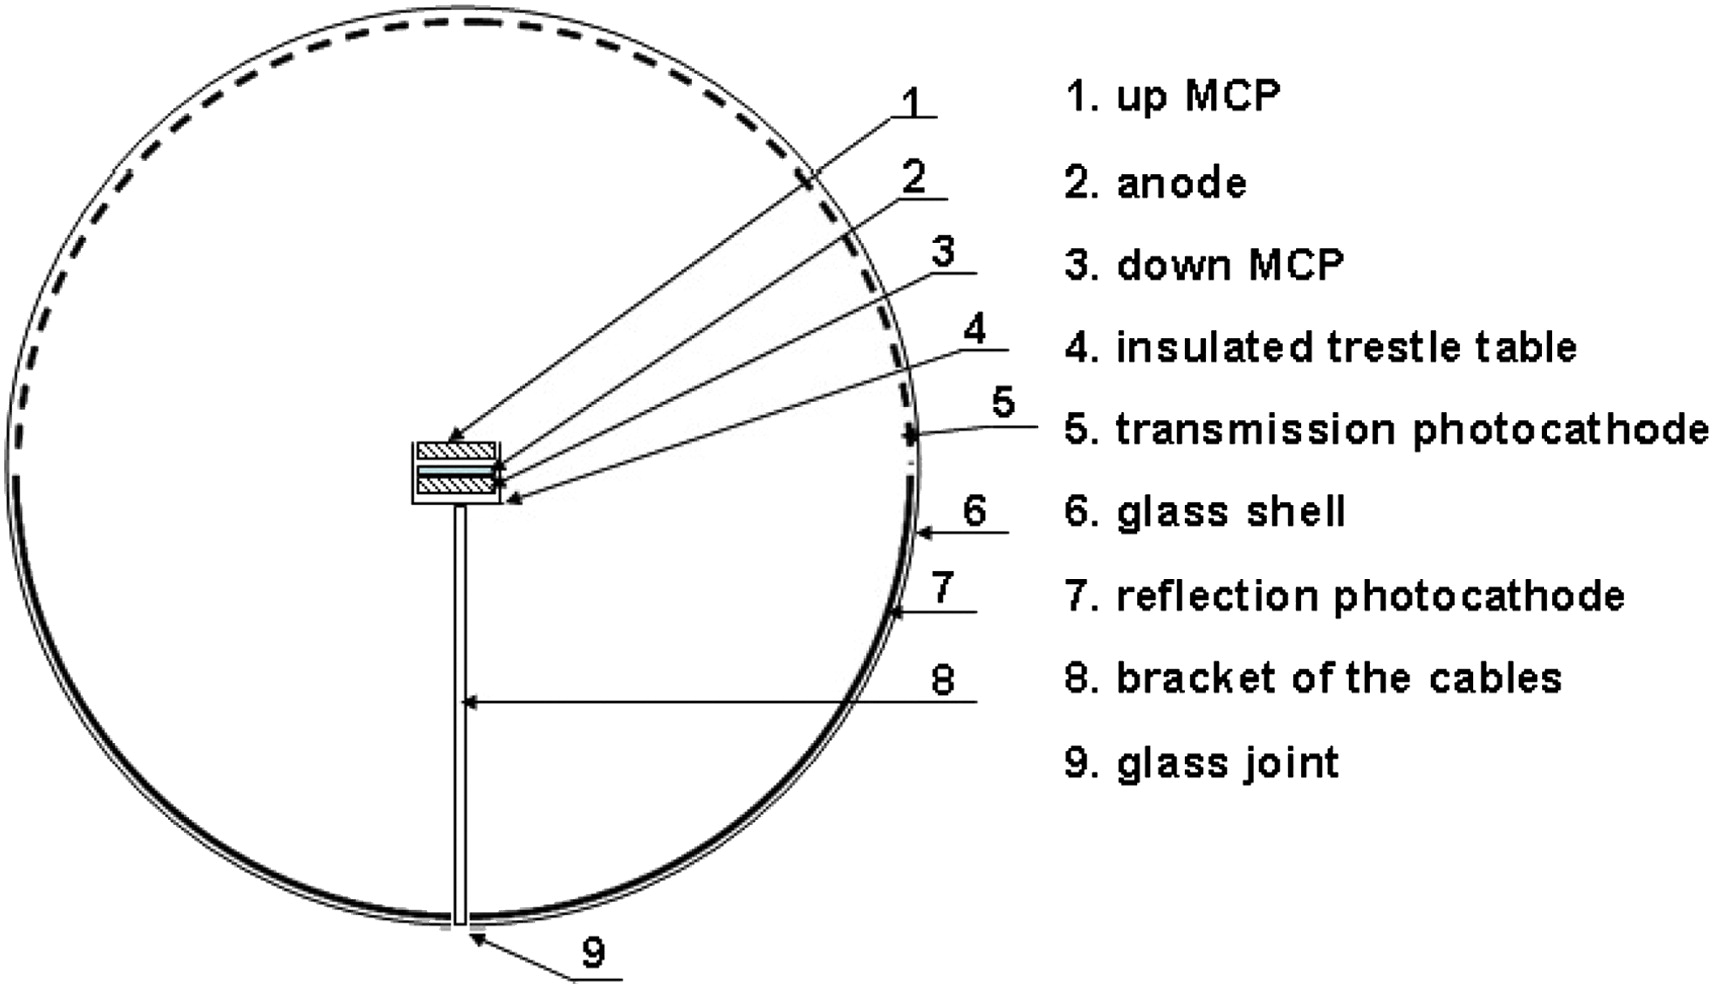
\includegraphics[width=0.75\linewidth]{scheme.jpg}
    \caption{MCP-PMT 的结构设计图\cite{wangNewDesignLarge2012}}
\end{figure}

在光子在 MCP-PMT 内部光阴极与材料发生相互作用产生光电子后,电子在椭圆形玻璃球壳内的电场作用下,向 MCP 迁移。
PMT 需要使用屏蔽线圈来抵消地磁场的影响,使得光电子能以尽量高的效率到达 MCP。
MCP 使用加高压的长通道实现电子加速,并以一定的小角度倾斜,使得电子容易与壁材料发生相互作用实现倍增,
同时又不使二次电子飞行轨迹与壁夹角过大致电子难以逸出。
MCP 的长通道截面积占横截面的比例称为开口比 $A$。

\begin{figure}
    \centering
    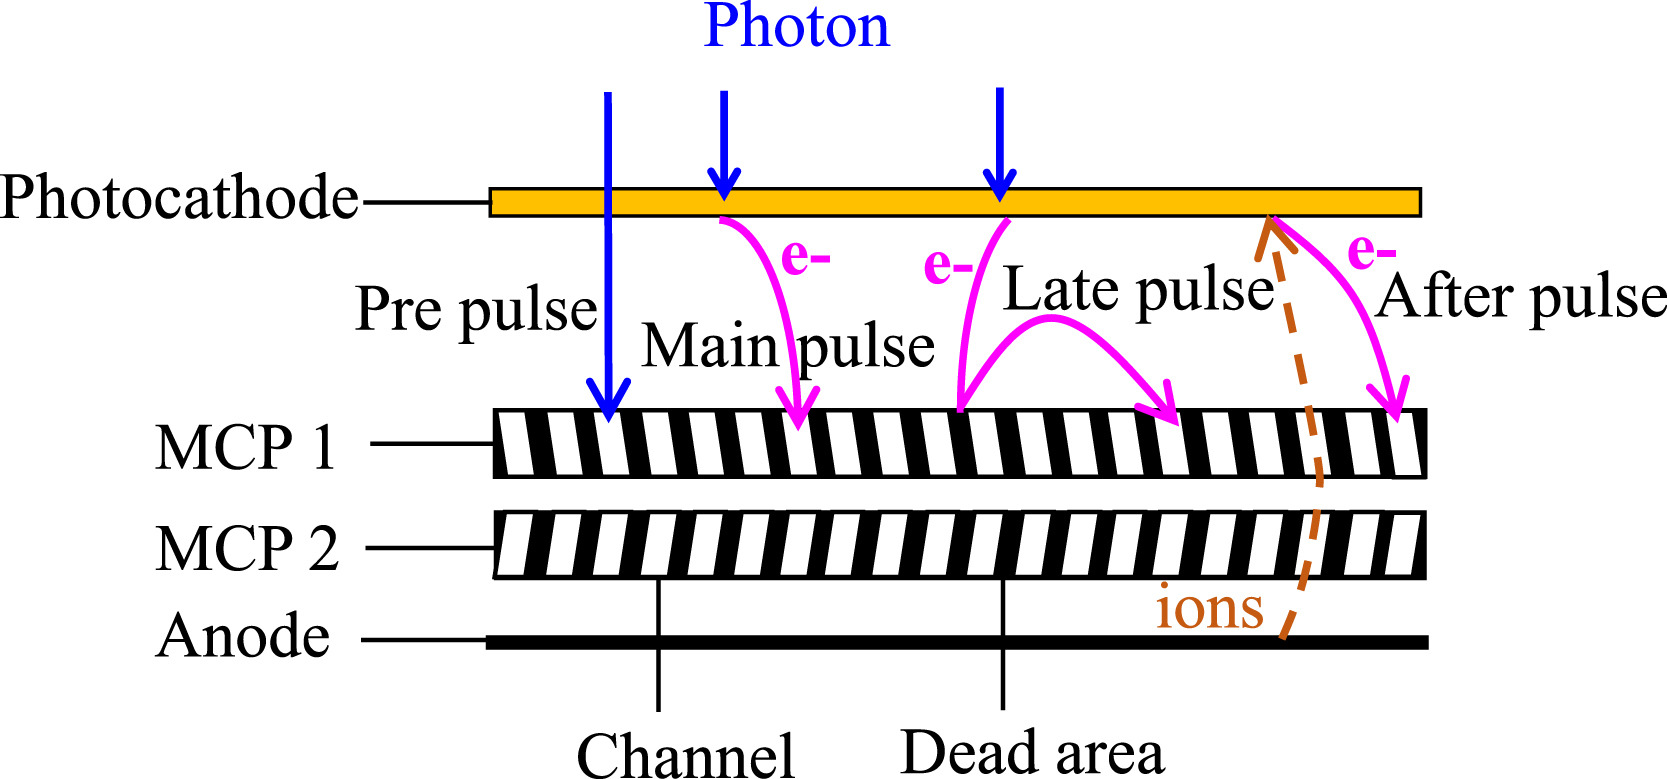
\includegraphics[width=0.85\linewidth]{process.jpg}
    \caption{MCP-PMT 中物理过程\cite{chenPhotoelectronBackscatteringMicrochannel2018}}
    \label{fig:pulses}
\end{figure}

MCP-PMT 的主要噪声来源为离子反馈\cite{MaterialStore2010}。即使 MCP-PMT 需要内部近似真空的工作条件,但仍存余少许的气体分子。
气体分子被电离,在高压电场中与倍增电子运动方向相反,既可能撞击壁产生二次电子被阳极收集,
也可能反向加速直至撞击光阴极,由于从产生到被收集的时间(渡越时间)较电子长,故将与主峰后形成次级脉冲,且还能够对光阴极材料造成损伤。
如果延长加速通道或者提高高压,这些脉冲也将得到放大,为了有效提高信噪比,常常使用两层 MCP 并使通道倾角对称。
由于在正离子与电子运动方向上引入了反角的设计,速度较小的反馈离子更难以进入与产生处对称的另一级 MCP,
从而有效提高信噪比,同时对电子再次倍增,获得较大的增益。

为了提高 CE 系数,最初在 MCP 入射处使用涂层(镍铬电极),使得入射的光电子可能能够在该表面进行倍增。
在后来的设计中,采用了 $\text{Al}_2\text{O}_3-\text{MgO}$ 复合涂层作为 ALD 涂层材料的方案,
起到提高二次倍增电子数 $\delta_{ts}$ 与延长寿命的作用。

在先前基于 Furman 模型\cite{PhysRevSTAB.5.124404}的模拟\cite{chenOptimizationElectronCollection2016}中,将光电子与涂层发生的相互作用分为三类:
\begin{itemize}
    \item 在涂层表面发生弹性散射;
    \item 进入涂层原子,发生散射而脱离涂层;
    \item 与涂层作用产生若干个能量较低的二级电子,亦称为真二次发射电子。
\end{itemize}

\begin{figure}
    \centering
    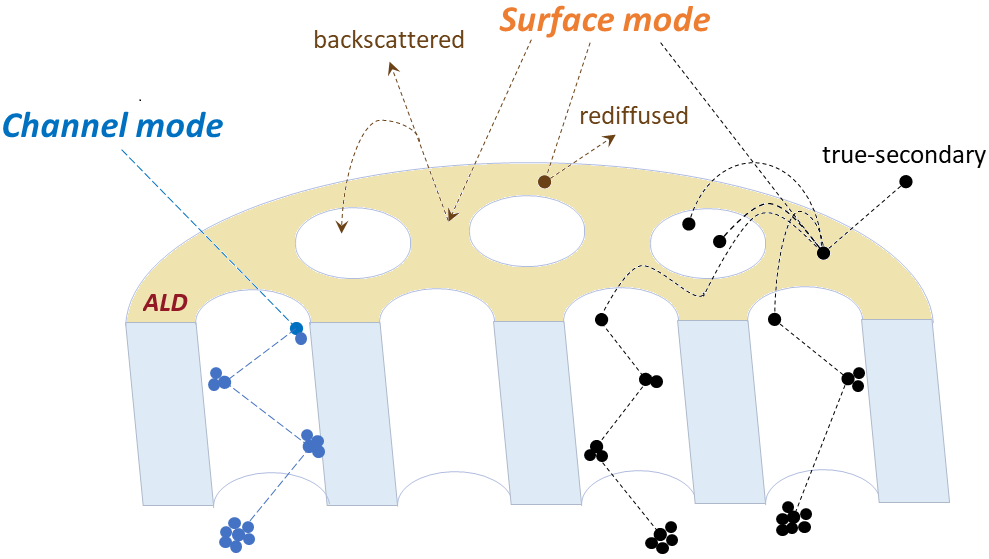
\includegraphics[width=0.85\linewidth]{mcp-pmt.png}
    \caption{光电子与 MCP-PMT 的三种相互作用形式}
\end{figure}

在三种模式中,发生前两种散射模式的单个光电子均只能产生一个光电子,而发生二次倍增的电子则可以产生自然数个真二次发射电子,
其个数 $\delta_{ts}$ 与入射电子能量 $E$、与涂层表面法线夹角 $\theta$ 存在依赖,由 Furman 模型给出:
\begin{equation}
    \delta_{ts}(E,\theta)=\hat{\delta}(\theta)D\left[\frac{E}{\hat{E}(\theta)}\right].
\end{equation}

其中 $\hat{\cdot}$ 代表 $\cdot$ 函数项的极值,$D(\cdot)$ 为一个满足 $D(1)=1,\ D^\prime(1)=0$ 的尺度函数,Furman 等人选择:
\begin{equation}
    D(x)=\frac{sx}{s-1+x^s}.
\end{equation}

其中 $s>1$ 为可调节变量。而对于二次倍增电子数服从的分布,Furman 等人给出了泊松分布与二项式分布两种选择,
其中二项式分布需要依据材料,选择对应的随机变量上限 $M$,在实际未知材料性质的情况下使用泊松分布是更合适的。

\subsection{单光电子电荷响应}\label{sec:spe-charge}
在 8 寸 MCP-PMT 的单光电子电荷响应研究\cite{wengSingleElectronCharge2024}中,电子进孔倍增的电荷响应采用 Gamma 分布描述。
这是因为在每一次倍增中,倍增电子的个数均服从泊松分布,并依次级联,
这种级联泊松最终可以用 Gamma 分布相较于其他常用分布(例如高斯分布)更好地近似。
相较于常用的高斯分布,Gamma 分布的另一个好处是在非正区间上概率密度严格为 0。

同时,真二次发射电子与其他未在涂层表面倍增而进入 MCP 倍增的电子相比,除了能量与到达阳极时间外没有本质区别,
其电荷响应亦使用 Gamma 分布描述。在 8 寸的仿真中,真二次发射电子的电荷被发现服从同一个 Gamma 分布 $\Gamma(\alpha_{ts}, \beta_{ts})$。
在~\ref{sec:mcp-pmt-process} 节中,Furman 模型给出真二次发射电子数目服从泊松分布的建议,因此真二次发射电子的电荷响应部分可以表示为:
\begin{equation}
    \left.
        \begin{array}{c}
        Q_\mathrm{ts}=\sum_{\mathrm{i=1}}^{\delta_{ts}}Q_\mathrm{i}\\
        \delta_{ts}\sim\pi(\lambda)\\
        Q_\mathrm{i}\sim\Gamma(\alpha_{ts},\beta_{ts})
        \end{array}
    \right\}\implies
    Q_\mathrm{ts}\sim\mathrm{Tw}_{\xi}
    \left(\mu(\boldsymbol{\theta_{ts}}),\sigma^2(\boldsymbol{\theta_{ts}})\right),\quad
    \boldsymbol{\theta_{ts}}=(\lambda, \alpha_{ts},\beta_{ts}).
    \label{eq:compound-poisson-gamma}
\end{equation}

即服从泊松分布个数的 Gamma 分布之和等价于指数参数 $\xi\in(1, 2)$ 的 Tweedie 分布。
Tweedie 分布是一种特殊的指数族分布,由 $\xi$ 调节分布的种类,由 $\mu$ 代表期望,由 $\phi$ 线性调节方差:
\begin{equation}
    Y\sim\mathrm{Tw}_{\xi}(\mu, \sigma^2)\implies 
    \left\{
        \begin{array}{c}
        \mathrm{E}[Y]=\mu \\
        \mathrm{var}[Y]=\phi\mu^{\xi}
        \end{array}
    \right.
    \label{eq:tweedie}
\end{equation}

~\eqref{eq:compound-poisson-gamma} 对比~\eqref{eq:tweedie},可得映射关系:
\begin{align}
    \xi & = \frac{2+\alpha_{ts}}{1+\alpha_{ts}}\\
    \mu & = \lambda\cdot\frac{\alpha_{ts}}{\beta_{ts}}\\
    \phi & = (1+\alpha_{ts})\left[\lambda\alpha_{ts}\beta_{ts}^{(1+\alpha_{ts})}\right]^{-\frac{1}{1+\alpha_{ts}}}
\end{align}

对于只在表面弹性散射或进入涂层材料原子核但被散射出涂层的电子,以及没有与涂层相互作用而直接进入 MCP 进行倍增的电子,
它们没有在涂层表面进行倍增,彼此的区别在于飞行径迹与 TT 不同,从而对 TTS 产生贡献。
它们在 MCP 中的倍增行为相同,电荷增益可以使用同一个 Gamma 分布 $\Gamma(\alpha, \beta)$ 来描述。
该分布作为单光电子进入 MCP 倍增的电荷结果,直接表示了 MCP-PMT 对单光电子的增益水平,
因此可以定义增益 $Q_1\equiv\frac{\alpha}{\beta}$ 与分辨率 $\eta\equiv\frac{\sqrt{\alpha/\beta^2}}{\alpha/\beta}=\frac{1}{\sqrt{\alpha}}$。

至此,MCP-PMT 的单光电子响应模型可以表示为:
\begin{equation}
    S(q)=p_0\Gamma(\alpha, \beta)+(1-p_0)\mathrm{Tw}_{\xi}
    \left(\mu(\boldsymbol{\theta_{ts}}),\sigma^2(\boldsymbol{\theta_{ts}})\right),\quad
    \boldsymbol{\theta_{ts}}=(\lambda, \alpha_{ts},\beta_{ts}).
\end{equation}

其中 $p_0$ 代表主峰的占比,它可以认为是所有未在涂层上进行真二次电子发射的原始电子的比例,
它与开口比、进孔比例、涂层材料性质等物理因素直接相关,可以视为级联伯努利事件的概率密度:
\begin{enumerate}
    \item 电子以 $p_{ch}$ 的概率进入 MCP 倍增,以 $1-p_{ch}$ 的概率撞击 MCP 表面 ALD 涂层
    \item 撞击 MCP 上表面的电子以 $p_{ts}$ 的概率进行真二次电子发射,以 $1-p_{ts}$ 的概率进入 MCP 进行倍增
\end{enumerate}

最终可以认为 $p_0=(1-p_{ch})\cdot(1-p_{ts})$。1. 中 $p_{ch}$ 应满足 $p_{ch}<A$,因为存在电场透镜效应,
电场线在平面上的孔隙处呈扩散状,对电子的运动有“发散”的作用,使得电子进入孔隙的概率变小。

8 寸研究中,指出 2. 中有 $p_{ts}\sim90\%$ 且在典型参数下应有 $p_{ts}>75\%$。
依据经验应有 $p_0<A$,关于 MCP-PMT 延迟脉冲的研究\cite{chenPhotoelectronBackscatteringMicrochannel2018}
指出在 $A=65\%$ 的情况下,应有 $p_0=55\%$。

在 8 寸研究中,对真二次倍增电子相对主峰的均值与标准差做出了限制建议:
\begin{align}
    \mu_{ts}&=\frac{\alpha_{ts}}{\beta_{ts}}\in[0.3, 0.7]\ Q_1\\
    \sigma_{ts}&=\sqrt{\frac{\alpha_{ts}}{\beta_{ts}^2}}\in[0.05, 0.3]\ Q_1
\end{align}

本研究中拟合均采取这一建议区间。

\section{分区间数据的拟合方法}
由于一次激光刻度取数中,电荷计数能够达到数万甚至数十万,
直接对每个计数进行拟合的内存消耗与效率极不理想。
如果能够以尽可能接近电荷模型原始概率分布的分区间方式,
将需要计算的计算点减少至数十至数百个,
将有约三个数量级的效率提升。

\subsection{分区间方法}
常用的分区间包括平方根方法、Sturges 公式、Rice 准则、Scott 准则、Terrell-Scott 准则、Doane 公式、Freedman-Diaconis 准则等。

\begin{table}
    \centering
    \caption{多种分区间方法的比较}
    \resizebox{\textwidth}{!}{
    \begin{tabular}{llll}
    \toprule
    方法 & 区间数 & 区间宽 & 优势与适用范围 \\
    \midrule
    平方根方法 & $k=\lceil\sqrt{n}\rceil$ & ------ & 简单 \\
    Sturges 公式 & $k=\lceil\log_2n\rceil+1$  & ------ & \makecell[l]{正态分布;\\样本数量适中} \\
    Rice 准则 & $k=\lceil2\sqrt[3]{n}\rceil$ & ------ & 简单 \\
    Scott 准则 & ------ & $h=\frac{3.49\hat{\sigma}}{\sqrt[3]{n}}$  & \makecell[l]{简单;\\正态分布} \\
    Terrell-Scott 准则 & $k=\sqrt[3]{2n}$ & ------ & \makecell[l]{渐进极小均方误差的积分;\\适用于非正态分布}   \\
    Doane 公式 & \makecell[l]{$k=1+\log_2(n)+\log_2\left(1+\frac{|g_1|}{\sigma_{g_1}}\right)$\\$g_1$偏度,$\sigma_{g_1}=\sqrt{\frac{6(n-2)}{(n+1)(n+3)}}$} & ------ & \makecell[l]{基于 Sturges 公式;\\适用于非正态分布} \\
    Freedman-Diaconis 准则 & ------ & \makecell[l]{$h=2\frac{\mathrm{IQR}(x)}{\sqrt[3]{n}}$\\IQR四分位距} & \makecell[l]{对离群值不敏感;\\适用于非正态分布} \\
    \bottomrule
    \end{tabular}}\label{tab:histogram}
\end{table}

在表~\ref{tab:histogram} 中,Freedman-Diaconis 准则既在系数部分使用了四分位距 IQR,
考虑了随机变量分布的偏度而避免像 Doane 公式一样直接计算偏度与其标准差,降低了计算难度,
又在幂次上同样渐进极小均方误差的积分\cite{freedmanHistogramDensityEstimator1981},
即 $k\propto n^{1/3}\ \simeq\ h\propto n^{-1/3}$,
确保在样本统计量大的情况下能够以最优的幂次还原原始概率分布。
综上所述,本研究中使用 Freedman-Diaconis 准则来对电荷计数进行分区间,再进行拟合。

\subsection{最小二乘法}
不妨约定 $q$ 为自变量,$q_i$ 表示第 $i$ 个直方图区间的自变量闭区间,
$n_i$ 表示第 $i$ 个直方图区间的实际计数,或称为频数,总事例数 $N=\sum_{i}n_i$;
$e_i$ 表示第 $i$ 个直方图区间的预期计数,或称为预期频数,可由下式给出:
\begin{equation}
    e_i(\boldsymbol{\theta}) = N\int_{\inf q_i}^{\sup q_i}\mathrm{d}q\cdot f(q;\boldsymbol{\theta})
\end{equation}

其中 $f(q;\boldsymbol{\theta})$ 代表在给定参数集 $\theta$ 时电荷谱的条件概率密度函数。

将直方图的每一个区间都视为一次测量,测量结果为频数,可以定义 $\chi^2(\boldsymbol{\theta})$:
\begin{equation}
    \chi^2(\boldsymbol{\theta})\equiv\sum_{i}\frac{\left[n_i-e_i(\boldsymbol{\theta})\right]^2}{\sigma_i^2}
    \label{eq:chi-sq}
\end{equation}

其中 $\sigma_i^2$ 代表第 $i$ 个直方图区间的频数的方差。
为了计算方差,使用预期频数 $e_i$ 替代方差 $\sigma_i^2$ 或使用频数 $n_i$ 替代方差 $\sigma_i^2$ 是两种可行的做法。

如果每个区间的计数 $n_i$ 相较总事例数 $N$ 占比小,可以认为渐进总事例数 $N$ 无穷、发生概率 $p$ 无穷小而 $Np$ 有限的泊松分布 $\pi(n_i;Np)$,
因此有近似 $\sigma^2_i=n_i$:
\begin{equation}
    \chi^2(\boldsymbol{\theta})=\sum_{i}\frac{\left[n_i-e_i(\boldsymbol{\theta})\right]^2}{n_i}
    \label{eq:pois-ls}
\end{equation}

如果将每个区间视为各自独立且具有较大数学期望的计数结果,则可近似认为服从高斯分布,
因其误差可以认为仅仅由统计涨落贡献,故具有方差与数学期望相等的特征,
即 $\sigma^2_i=e_i$:
\begin{equation}
    \chi^2(\boldsymbol{\theta})=\sum_{i}\frac{\left[n_i-e_i(\boldsymbol{\theta})\right]^2}{e_i}
    \label{eq:gauss-ls}
\end{equation}

根据大数定律,这两种近似在样本量趋近无穷时,具有相同的极限,但它们在有限样本量下的取舍则有所不同:
\begin{itemize}
    \item~\eqref{eq:pois-ls} 需要每个区间事例数占比都较小;
    \item~\eqref{eq:gauss-ls} 需要每个区间事例数足够多,尤其不能为空,否则不能良定义。
\end{itemize}

在本研究中,发现按照 Freedman-Diaconis 准则划分的直方图中,计数最多的区间计数可达总计数的 20\%,
因此~\eqref{eq:pois-ls} 假设并不成立,且由于每个区间计数较多,
选用~\eqref{eq:gauss-ls} 作为极小化的函数是合适的。

关于拟合结果的误差分析,最准确的办法是对一系列的自变量 $\boldsymbol{\theta}$ 做 Monte Carlo 模拟,
得到 $\chi^2$ 的概率密度分布,从而得到拟合得到 $\chi^2$ 的置信区间,作为该模型的合理性定量依据。
在我们认为每个区间计数较多的前提下,上文已经表明每个区间计数可以认为服从高斯分布,
从而可以近似认为拟合得到的 $\chi^2$ 结果服从卡方分布,得到模型的合理性估计。

\subsection{极大似然法}
同样约定 $q$ 为自变量,$q_i$ 表示第 $i$ 个直方图区间的自变量闭区间,共有 $m$ 个区间,
$n_i$ 表示第 $i$ 个直方图区间的频数,总事例数 $N=\sum_{i}^{m}n_i$,$\boldsymbol{n}=(n_1, n_2, \ldots, n_m)$ 代表各区间的频数向量,
$e_i$ 表示第 $i$ 个直方图区间的预期频数,各区间预期频数使用 $\boldsymbol{e}$ 表示,可由下式给出:
\begin{equation}
    e_i(\boldsymbol{\theta}) = N\int_{\inf q_i}^{\sup q_i}\mathrm{d}q\cdot f(q;\boldsymbol{\theta})
    \label{eq:ei}
\end{equation}

可见存在函数满足参数集 $\boldsymbol{\theta}$ 至预期频数 $\boldsymbol{e}$ 之间的双射。
各区间事例数 $\boldsymbol{n}$ 可以视为总数为 $N$ 的 $m$ 次多项式分布结果,在该处的概率分布密度为:
\begin{equation}
    \begin{aligned}
        P(\boldsymbol{n},\boldsymbol{e}|\boldsymbol{\theta})
        &=P(\boldsymbol{n}|\boldsymbol{\theta})\\
        &=\frac{N!}{n_1!\cdots n_m!}\left[\frac{e_1(\boldsymbol{\theta})}{N}\right]^{n_1}
        \cdots\left[\frac{e_m(\boldsymbol{\theta})}{N}\right]^{n_m}\\
        &=\frac{N!}{n_1!\cdots n_m!}\cdot\frac{\prod_{i=1}^{m}e_i^{n_i}(\boldsymbol{\theta})}{N^N}
    \end{aligned}
    \label{eq:hist-pdf}
\end{equation}

对~\eqref{eq:hist-pdf} 取对数得:
\begin{equation}
    \begin{aligned}
        \ell&=\ln P(\boldsymbol{n}|\boldsymbol{\theta})\\
        &=\sum_{i=1}^{m}n_i\ln{e_i(\boldsymbol{\theta})}
        +\ln{N!}-\sum_{j=1}^{m}\ln{n_j!}-N\ln{N}\\
        &=\sum_{i=1}^{m}n_i\ln{e_i(\boldsymbol{\theta})}+C
    \end{aligned}
    \label{eq:log-l}
\end{equation}

其中 $C$ 代表与自变量 $\boldsymbol{\theta}$ 无关的常数,在极大似然过程中对结果没有影响。
极大似然法相较于最小二乘法,不需要做出近似假设,且对各区间频数 $n_i$ 没有要求,
始终具有良定义,但由于需要计算对数,计算开销更大,在复杂电荷模型的假设下优化更加困难。

\section{傅里叶变换带光强电荷模型}\label{sec:fourier}
出于三个原因,考虑光强的刻度方法有被引入的必要性:
\begin{enumerate}
    \item 在 PMT 的刻度与实际运行中,可能遇到光强较强以至于多个光电子情形不可忽略甚至占主要成分的情况;
    \item 由于本研究所考虑的 MCP-PMT 相较于传统打拿级 PMT,具有电荷长尾的效应,
    实际电荷谱上较主峰能道高的区域由单光电子模型中 Tweedie 成分与多光电子的主峰共同贡献;
    \item 对于低光强的刻度数据,大统计量的 0 电荷计数被排除在单光电子谱刻度外,没有得到充分利用。
\end{enumerate}

拟合引入 0 电荷计数,能够极大提高统计量,得到相对误差较小的光强,
从而在电荷谱的能道较高范围内尽可能消除多光电子的贡献对长尾参数的影响,
提高目标 MCP-PMT 的增益刻度准确性。

\subsection{任意光电子数电荷谱}\label{sec:dft}
光电子个数服从期望为 $\mu$ 的泊松分布,即:
\begin{equation}
    P(\text{PE}=n) = \pi(n;\mu)=\sum_{i=0}^{+\infty}\frac{\mu^{n}}{n!}\cdot e^{-\mu}
\end{equation}

当光电子个数为 0 时,考虑到没有光电子时的电荷应该严格为 0,电荷谱密度可以认为是:
\begin{equation}
    S_{0\text{PE}}(q)=N_{0\text{PE}}\cdot\delta(q)=\pi(0;\mu)\cdot\delta(q)
\end{equation}

当光电子个数为正整数 $k\in\mathbb{N}^{+}$ 时,电荷谱密度等效于 $k$ 个单光电子谱卷积:
\begin{equation}
    \begin{aligned}
        S_{k}(Q = \sum_{i = 1}^{k} q_i ) 
        & = \pi(k;\mu)\cdot\underbrace{
        \int_{-\infty }^{+\infty}\mathrm{d}q_1\cdot S(q_1)
        \cdots \int_{-\infty }^{+\infty}\mathrm{d}q_k\cdot S(q_k)
        }_{k}\\
        &=\pi(k;\mu)\cdot\underbrace{S(q)\otimes\cdots\otimes S(q)}_{k}.
    \end{aligned}
    \label{eq:kpe-charge}
\end{equation}

其中 $S(q)$ 为单光电子电荷谱概率密度函数。傅里叶变换 $\mathcal{F}$ 能够将卷积变为另一个域上的直积:
\begin{equation}
    \mathcal{F}\left[f(t)\otimes g(t)\right]=\mathcal{F}[f(t)]\cdot\mathcal{F}[g(t)].
    \label{eq:fourier}
\end{equation}

因此对~\eqref{eq:kpe-charge} 做傅里叶变换并对 $k\in\mathbb{N}^{+}$ 求和即得正整数个光电子时的电荷谱密度为:
\begin{equation}
    \tilde{S}_{\ge1\text{PE}}(p)=\sum_{k=1}^{\infty}
    \pi(k;\mu)\cdot\tilde{S}^k(p).
    \label{eq:pe-charge}
\end{equation}

其中 $\tilde{\cdot}(p)$ 代表函数 $\cdot$ 经过 $\mathcal{F}$ 后在另一个数域 $\{p\}$ 上的数值。
考虑~\eqref{eq:pe-charge} 补全 0 个光电子时的无穷级数求和:
\begin{equation}
    \begin{aligned}
        \tilde{S}_{\ge1\text{PE}}(p)
        &=\sum_{k=0}^{\infty}\pi(k;\mu)\cdot\tilde{S}^k(p)-\pi(k;\mu)\\
        &=\sum_{k=0}^{\infty}\frac{e^{-\mu}}{k!}\cdot\left(\mu\tilde{S}(p)\right)^k-e^{-\mu}\\
        &=e^{\mu(\tilde{S}(p)-1)}-e^{-\mu}\\
        &=e^{-\mu}(e^{\mu\tilde{S}(p)}-1).
    \end{aligned}
    \label{eq:postive-charge}
\end{equation}

通过傅里叶变换,能够将任意多个光电子的卷积分布转化为另一个定义域上的直积,
并借助泊松分布的性质实现解析求和,既不需要截断无穷级数求和,也不需要计算卷积,
是完全无损失的理论方法,因此得到的参数应是无偏的。

考虑 0 电荷处的概率密度则需要综合考虑 0 个光电子与单光电子中 Tweedie 成分的贡献:
\begin{equation}
    \begin{aligned}
        S_{\text{total}}(q=0)
        &=S_{\ge1\text{PE}}(q=0)+S_{0\text{PE}}(q=0)\\
        &=\sum_{k=1}^{\infty}\pi(k;\mu)\cdot S^k(q=0)+\pi(0;\mu)\\
        &=\sum_{k=0}^{\infty}\pi(k;\mu)\cdot S^k(q=0)\\
        &=\sum_{k=0}^{\infty}\frac{e^{-\mu}}{k!}\cdot\left[\mu S(q=0)\right]^k\\
        &=\sum_{k=0}^{\infty}\frac{e^{-\mu}}{k!}\cdot\left[\mu(1-p_0)e^{-\lambda}\right]^k\\
        &=e^{\mu\left[(1-p_0)e^{-\lambda}-1\right]}.
    \end{aligned}
    \label{eq:zero-charge}
\end{equation}

\subsection{复合 Simpson 数值积分}
借助~\ref{sec:dft} 所述的方法,一组参数已经能够利用 FFT 与 IFFT 映射到一系列采样点上的概率密度函数值。
为了得到原电荷谱上特定区间内的预测频数,需要使用数值积分方法。
常用的数值积分方法包括:矩形法,Lagrange 插值法与 Newton-Cotes 插值法等,
在此不展开介绍各方法的应用场景与变形。

复合 Simpson 积分法是 Newton-Cotes 插值法的特殊形式,特别适用于间隔给定的特定区间上的数值积分。
其具体计算方式如下:
\begin{equation}
    \begin{aligned}
        \int_{a}^{b}f(x) dx
        &=\sum_{i=1}^{n/2}\frac{h}{3}\left[f(x_{2i-2})+4f(x_{2i-1})+f(x_{2i})\right]-\frac{f^{(4)}(\xi_i)}{90}h^5 \\
        &=\frac{h}{3}\left[f(x_0)+4f(x_1)+2f(x_2)+\cdots+2f(x_{n-2})+4f(x_{n-1})+f(x_n)\right]
        -\frac{h^2}{90}\sum_{i=1}^{n/2}f^{(4)}(\xi_i) \\
        &=\frac{h}{3}\left[f(x_{0})+4\sum_{i=1}^{n/2}f(x_{2i-1})+2\sum_{i=1}^{n/2-1}f(x_{2i})+f(x_{n})\right]
        -\frac{h^2}{90}\sum_{i=1}^{n/2}f^{(4)}(\xi_i).
    \end{aligned}
    \label{eq:simpson}
\end{equation}

其中 $x_i$ 为等间距 $h$ 的序列满足 $a=x_0<x_1<\cdots<x_n=b$。
考虑连续函数 $f^{(4)}(\xi)$ 的介值定理,应有:
\begin{equation}
    \frac{2}{n}\sum_{i=1}^{n/2}f^{(4)}(\xi_i)=f^{(4)}(\xi),\quad\xi\in\left[\min(\xi_i), \max(\xi_i)\right].
\end{equation}

依此给出~\eqref{eq:simpson} 的误差项为 $-\frac{nh^5}{180}f^{(4)}(\xi)=-\frac{(b-a)h^4}{180}f^{(4)}(\xi)$,
与原函数的四阶导数成正比,因此当且仅当对于三次及以下多项式,其误差严格为 0,或称为代数精度为 3。

复合 Simpson 积分法只需要使用特定点的函数值,在细分区间较多、每段区间较平滑的函数上,它的表现良好,
因此在本实验中采样点函数值到原电荷谱区间频数的预测均使用复合 Simpson 积分法计算。
为了尽可能减小误差,需要采样点间隔 $h$ 尽可能小。
Freedman–Diaconis 准则给出的区间宽 $h\propto n^{-1/3}$,
对于统计量越大的电荷刻度数据,原电荷谱的分区间数越大、间距越小,复合辛普森积分法效果越好。

\subsection{傅里叶变换的准确度与性能}
计算机并不能够对连续的 $S_{\text{total}}(q)$ 函数进行傅里叶变换,只能够使用有限离散傅里叶变换(Discrete Fourier Transformation,以下简称 DFT)对其进行近似,
并使用逆有限离散傅里叶变换(Inverse Discrete Fourier Transformation,以下简称 IDFT)。
应当从准确度与性能方面进行考量。

DFT 与 IDFT 结合的方法能够在离散距离趋近于无穷小时的极限为连续傅里叶变换与其逆变换,因此当采样间隔足够小时,即可实现理想的近似。
合适的间隔应当由定理~\ref{theo:shannon} 决定:
\begin{theorem}[Nyquist–Shannon 采样定理]\label{theo:shannon}
    对于具有带宽限制(即傅里叶变换后频率在有限区域以外为零)例如频率上限为 $f_s$ 的连续信号,使用周期冲激序列进行采样,
    若要完全还原初始连续信号的信息而不发生混叠,则应以不低于 $2f_s$ 的频率进行采样。
\end{theorem}

在实际中,由于连续函数的傅里叶变换常常不具有带宽限制,可以设定频率阈值下限,只需要满足采样频率至少高于该阈值对应频率的二倍,
原始连续信号的主要信息就能够被还原。在本研究中,将依据 Freedman–Diaconis 准则划分的电荷谱区间继续细分至 32 份后,
再增加区间已经没有可以显著观测的变化,可以认为已经理想地还原了原始连续电荷谱的信息。

快速傅里叶变换(Fast Fourier Transformation,以下简称 FFT,逆算法同理简称 IFFT)是一种 DFT 的高效算法,利用了 DFT 中系数的对称性与周期性,
能够将朴素 DFT 算法的 $O(n^2)$ 时间复杂度降低到 $O(n\log{n})$,对于本研究中每个 MCP-PMT 数万至数十万的统计量表现出显著的优势。

综上所述,傅里叶变换刻度方法的本质优势为避免卷积与无穷级数求和的时间复杂度与精度损失,
而使用较多的采样点,同时满足数值积分、FFT 与 IFFT 准确度的要求,
只需要付出较为廉价的内存代价,是理想的升级。

\section{刻度方法}

\subsection{电荷谱截断预处理}\label{sec:cut}
PMT 中存在部分巨大脉冲,是由 $\mu$ 子穿过 PMT 玻璃时发射的切伦科夫光与天然放射性本底造成的\cite{zhangStudy20inchPMTs2022}。
具体地,根据脉冲幅值,可以将划分为 PMT 的噪声计数主要来源分为三类\cite{zhangDarkCount20inch2024}:
\begin{itemize}
    \item $0\sim10$ mV,主要由热致电子发射(暗噪声)贡献;
    \item $10\sim100$ mV,主要由天然放射性贡献;
    \item $100\sim500$ mV,主要由 $\mu$ 子致切伦科夫光贡献。
\end{itemize}

在实际电荷谱中,除了主要事例(暗噪声、激光等)对应的电荷响应,还存在由 $\mu$ 子与天然放射性本底贡献的电荷,且集中在电荷较大的区域。
由于其对主峰后能道较高区域有贡献,因此需要引入一个电荷谱拟合时的上限截断。

在还原山体、玻璃器材中包含的 $^{238}\text{U}\ /\ ^{232}\text{Th}\ /\ ^{40}\text{K}$ 含量与未灌装水之前的实验条件下,
能够得到模拟结果,如图~\ref{fig:cut} 所示。

\begin{figure}
    \centering
    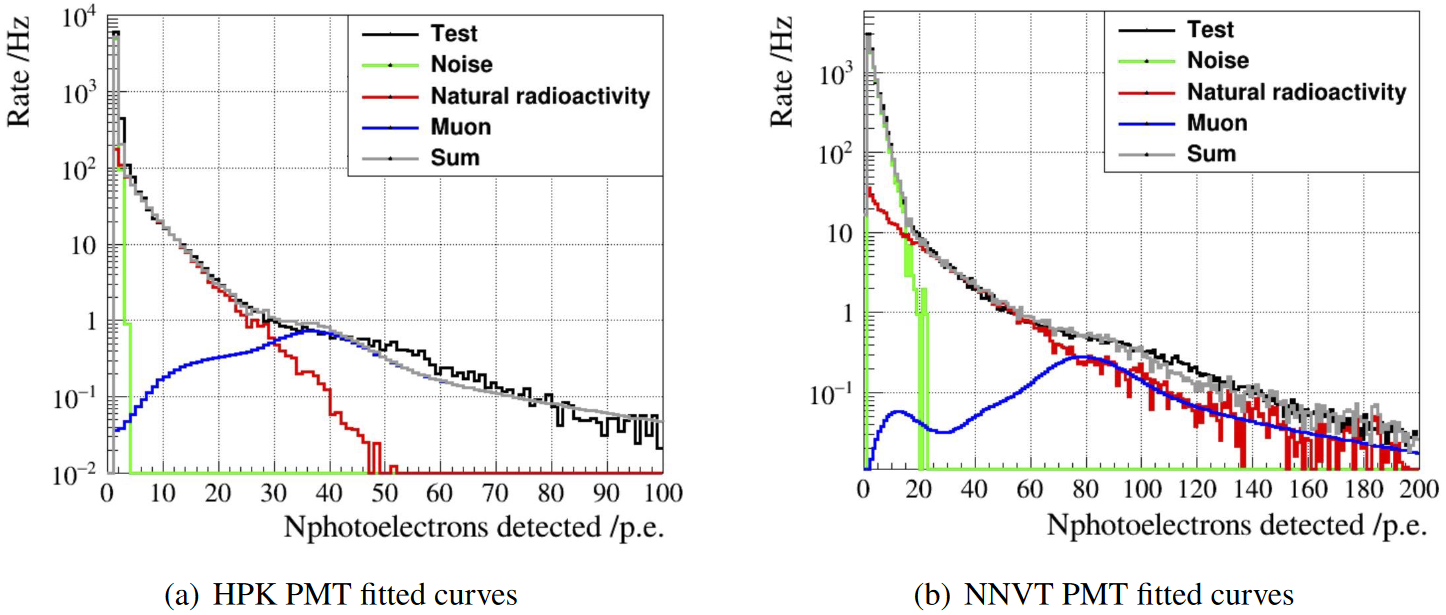
\includegraphics[width=\linewidth]{cut.png}
    \caption{Dynode PMT 与 MCP-PMT 各本底计数率\cite{zhangStudy20inchPMTs2022}}
    \label{fig:cut}
\end{figure}

对于不同的数据集应当采取不同的策略。对于暗噪声采数,暗噪声计数率约 $10\sim50$ kHz,但由于阈值较高(通常有至少 3 个或 7 个或 20 个 PMT 同时过阈才记录波形的设置),
按照暗噪声 50 kHz、偶然符合时间窗 50 ns 的假设进行估计,四重及以上偶然符合计数率有 $f_{coin}\ll1\enspace\text{Hz}$,实际触发率较低,
因此暗噪声的电荷计数主要由三重及以下符合贡献。
依据图~\ref{fig:cut} 可认为在 4 倍单光电子(photoelectron 或 PE)水平下暗噪声触发率接近其他本底的 20 倍左右,可以认为成分较为单一。

对于激光等光源采数,例如 OSIRIS 现场激光刻度触发率为 1.5 kHz,单脉冲的期望水平为 $\mu=0.01$ PE\cite{junocollaborationDesignSensitivityJUNO2021},
对于~\ref{sec:osiris} 节中位于赤道平面上的激光调制位于 $75\%\sim78\%$ 强度,光电倍增管平均光子探测效率为 29.1\%\cite{JUNOPhysicsDetector2022},
可以估计单激光通道下 PMT 接受 PE 频率期望为 3.3 Hz,即 PE 光子数服从强度为 3.3 的时齐泊松过程,
这与现场单激光通道采数 $\sim2\times10^{3}\enspace\text{PE}\ /\ 12\enspace\text{m}$ 的采数率符合。
此时暗噪声也属于本底,但信噪比相较暗噪声采数仍较优,此时预计 5 PE 较为合适。

已经完成的模拟研究中对于 PMT 工作环境的考虑并不完全,仍然需要考虑灌装水与灌装液体闪烁体后的其他本底水平。
灌装后水能够进一步屏蔽周围岩石、玻璃的放射性传播,因此天然放射性项在已经灌装水的探测器中影响将被削弱。

液闪中的 U/Th 等元素及其衰变链的活度受到严格控制,但在循环过程中会引入氡,经过 3 次液体闪烁体循环后,
OSIRIS 内部 $^{214}\text{Bi}-^{214}\text{Po}$ 特征事例的事例率 $\sim2\times10^{-3}\enspace\text{Hz}\ /\ 20\enspace\text{m}^3$ 
升至 $\sim1\times10^{-1}\enspace\text{Hz}\ /\ 20\enspace\text{m}^3$,
在 OSIRIS 探测器中相较于激光刻度采数的频率有 30 倍差距,但在 JUNO 中央探测器中这一比例将更微弱,
因此尤其是 JUNO 中央探测器需要在液体闪烁体循环后氡几乎消耗殆尽时再进行激光采数。

本研究中使用 OSIRIS 的激光刻度数据,综合考虑各本底,选取较简单的 5 倍主峰截断来近似 5 倍 PE 截断。

\subsection{评价指标}\label{sec:criterion}

定义自由度 ndf 为数据点数与模型参数个数之差,对于样本来自于高斯分布的情况,$(\chi^2,\text{ndf})$ 服从卡方分布:
\begin{equation}
    p(\chi^{2},n)=\frac{1}{2^{n/2} \Gamma(n/2)}[\chi^{2}]^{n/2-1}e^{-\chi^{2}/2},\quad0\leq\chi^{2}\leq\infty 
    \label{eq:chi-distribution}
\end{equation}

该种方法称为卡方检验,适用于拟合性检验与独立性检验。
特别地,在 $n\rightarrow\infty$ 时,$\chi^2$ 趋近于自由度为 $n-1$ 的卡方分布。
基于 $\alpha$ 显著性水平,定义 $\chi_\alpha^2$ 为关于 ndf 的临界函数,作为检验的卡方依据。

对于拟合性检验,存在更直接的指标:$\chi^2/\text{ndf}$。~\eqref{eq:chi-sq} 指出 $\chi^2$ 代表数据点偏差平方与方差的比值,
它与自由度 ndf 的比值代表平均意义上每个自由度拟合的相对偏差,在数据点较多的情况下也可近似为每个数据点拟合的相对偏差。
一般可以认为 $\chi^2/\text{ndf}\le1$ 为极优的拟合,$\chi^2/\text{ndf}=3\sim5$ 为较好的拟合。

% !TeX root = ../thuthesis-example.tex

\chapter{结合波形分析的迭代刻度方法}

\section{快速随机匹配追踪算法}\label{sec:fsmp}
探测器中发生的事件光学或带电粒子信号完全依靠 PMT 读出,当短时间(例如单光电子电压波形半高宽时间窗)内只有一个光电子到达 PMT,
则在相同的工作条件下,不同 PMT 具有相同的增益数量级,都能输出形状相似的负极性脉冲。然而,当至少两个光电子到达时,
各光电子响应的电压波形将堆积,使得光电子的个数与各自的能量、到达时间分辨难度提高。
面对该问题,有两种常用的技术手段:
\begin{enumerate}
    \item 以光电子波形到达前的一段波形计算本底信号的输出电压水平(基线),并将光电子波形积分得到电荷信息,
    使用经验换算关系得到光电子数并反推能量关系,时间信息则取波峰的特定上升沿(通常为 10\%)时刻为到达时间;
    \item 使用经验的单光电子波形,与去除基线的波形做反卷积,得到各光电子的到达时间。
\end{enumerate}

对于方法 1,由于前一个时间窗口的靠后位置可能存在信号脉冲,或脉冲的后延平稳电压水平与基线不同,电荷积分的区域不容易
形成一致共识。同时,每个光电子倍增后的电荷也具有概率分布,而方法 1 只能通过经验关系换算得到光电子数,无法得到其期望与方差,
因此对提高能量分辨率没有帮助。而对于时间分辨率,由于不同光电子波形的堆叠,方法 1 没有办法准确地区分出各个光电子的到达时间,
从而在事例重建的位置分辨率上也存在客观缺陷。

对于方法 2,对于不同的 PMT 与不同的工作电压,由于电场、渡越速度、噪声本底的水平不同,单光电子波形的幅值与展宽均有差异。
如果全部使用经验单光电子波形进行反卷积,得到的光电子数量与时间将分别由幅值与展宽的有偏估计引入偏差,从而减低事例重建的
能量分辨率与位置分辨率。

为了实现事例重建的能量分辨率与位置分辨率提升,需要一个贝叶斯方法,使得能够在不同的单光电子数量、到达时间、电荷样本空间
(这些空间是维度可变的)与单光电子响应波形找到最优解并给出误差分析。

快速随机匹配追踪算法(Fast Stochastic Matching Pursuit,以下简称 FSMP)\cite{wangFastStochasticMatching2024a}
是一种可逆跳跃的马尔可夫链蒙特卡罗方法(Reversible Jump Markov Chain Monte Carlo),能够在不同维度的样本空间内采样,
利用 Metropolis-Hastings 等采样方法,实现采样结果的跳跃(马尔可夫链状态的转移),最终收敛至马尔可夫链的稳态分布。

\begin{figure}
    \centering
    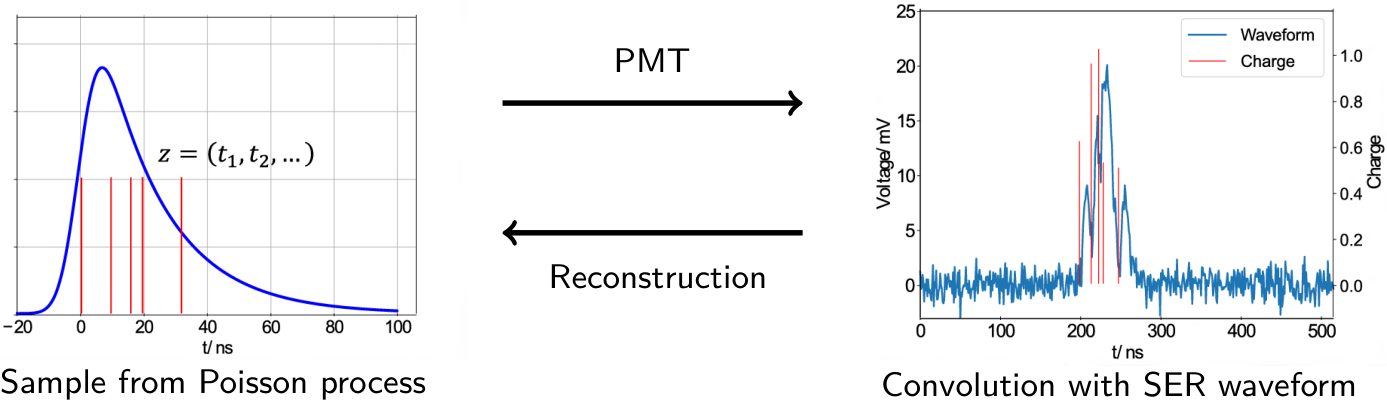
\includegraphics[width=.95\linewidth]{fsmp.png}
    \caption*{在 PMT 中,光电子的序列,在考虑增益与单电子响应波形卷积后形成波形;FSMP 能在不同样本空间采样,最终得到与波形最匹配的参数对。}
    \caption{FSMP 波形分析方法}
\end{figure}

针对 dynode PMT,该方法认为单光电子电荷服从高斯分布,光电子数服从泊松分布,因此波形中电荷的概率分布模型为复合泊松-高斯分布。
针对 MCP-PMT,该方法将单光电子电荷模型分解为若干个高斯分布线性之和,用以表示光电子在涂层表面不同行为的分类,
每一种高斯分布具有各自独立的期望与方差。

该方法在使用单高斯电荷响应的前提下,于模拟数据集与 8 寸 MCP-PMT 激光测试的实际数据集上均得到了应用与验证,已经获得了能量与时间分辨率的提升。
该工作给出结论,在兆电子伏特的液体闪烁体中微子探测中,该方法在理想情况下,可以提高可见能量的分辨率12\%。

\section{迭代刻度}
FSMP 波形分析方法可以得到光电子携带电荷信息,作为刻度的电荷谱输入,因此刻度需要依赖波形分析。
同时,如~\ref{sec:fsmp} 中所述,FSMP 同样依赖电荷模型作为采样依据,因此波形分析同样需要依赖刻度。
在波形分析与刻度结果相互依赖的客观条件下,为了使得刻度与波形分析的结果同时趋近真值,需要波形分析与刻度交替进行
并相互作为输入,直至物理结果收敛,则认为收敛到了贝叶斯后验解。

在没有进入迭代时,即使 MCP-PMT 的电荷谱只使用主峰均值作为波形分析的电荷模型输入,已经在实际激光波形上取得了理想的波形拟合效果,
得到的 TTS 从 $(1.719\pm0.001)$ ns 减小到 $(1.703\pm0.007)$ ns\cite{wangFastStochasticMatching2024a}。
借助波形分析与刻度迭代进行的工作方法,预期将能获得接近物理真值的 MCP-PMT 参数与实际波形的光电子信息,
对准确描述和利用 MCP-PMT 特性、发挥 FSMP 的能量与时间分辨率优势具有重要意义。

\subsection{时间窗筛选电荷}
FSMP 需要一系列相似发光曲线来实现迭代,因此暗噪声与放射源刻度为理想的刻度源。
如~\ref{sec:cut} 节所述,激光信噪比较暗噪声高,且持续时间短、脉冲波形形状相似,是理想的迭代数据集。
经过对 FSMP 分析得到的光电子数做生成率归一化后能够得到光变曲线。

\begin{figure}
    \centering
    \subcaptionbox{暗噪声光变曲线}
      {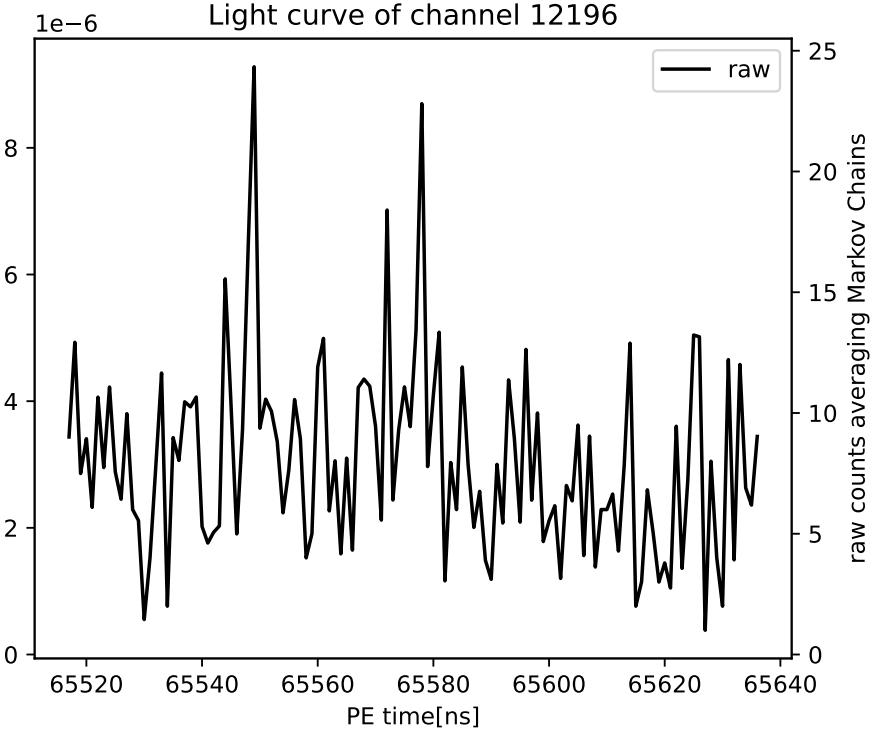
\includegraphics[width=0.47\linewidth]{lc_dcr.png}}
    \subcaptionbox{激光光变曲线}
      {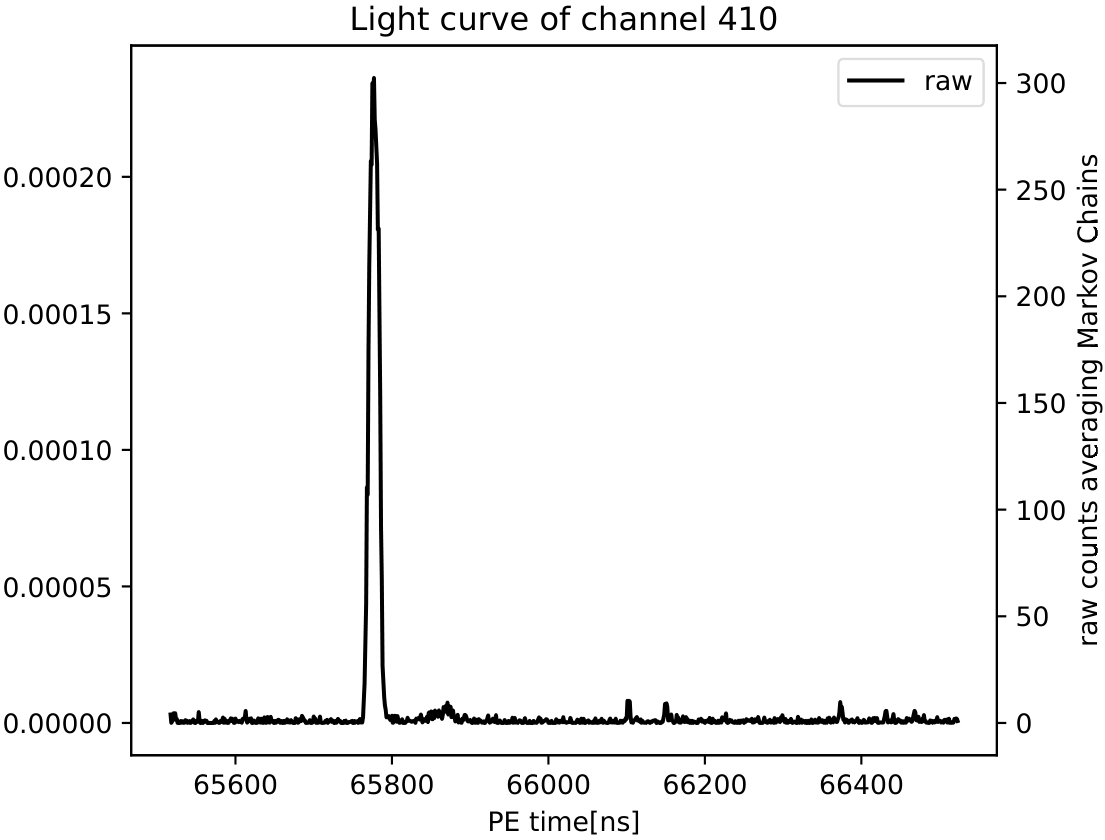
\includegraphics[width=0.51\linewidth]{lc_laser.png}}
    \caption{20 寸 MCP-PMT 在不同数据集上的光变曲线}
\end{figure}

由于光源与目标 PMT 相对位置的不同,因此光电子到达时间峰的时间存在偏差。为了保证各 PMT 的光变曲线相似,需要对时间窗筛选,
本研究中选择与波形预处理相似的 10\% 峰值决定上升下降时间,以此为光电子到达时间的接受区间,选择该部分光电子的电荷作为电荷谱进行拟合。

\begin{figure}
    \centering
    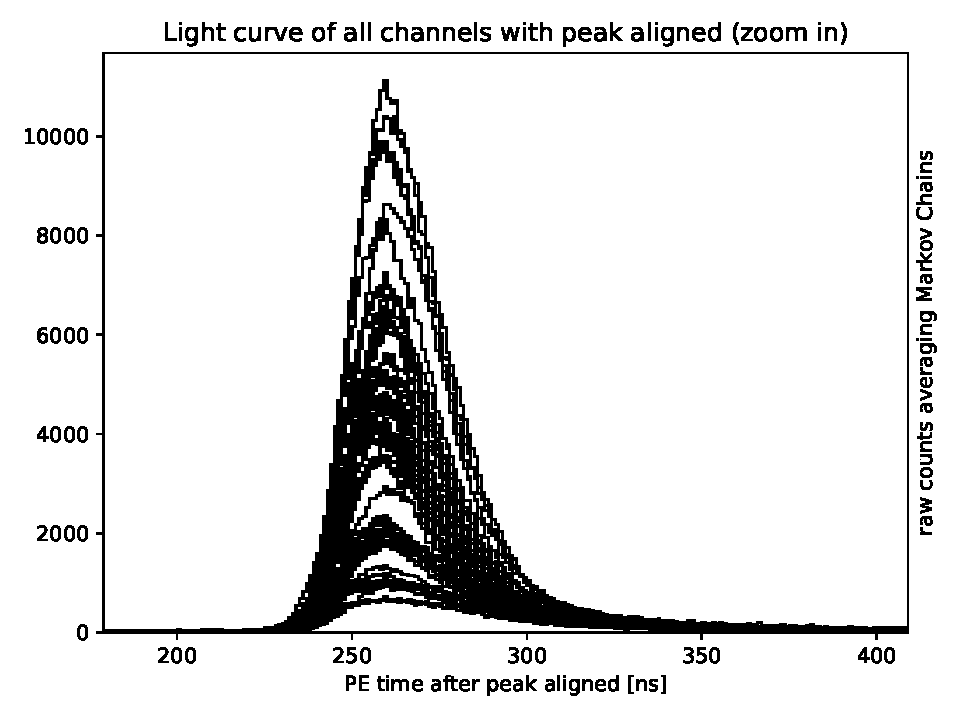
\includegraphics[width=.8\linewidth]{160109-3.pdf}
    \caption{峰对齐后的光变曲线}
    \label{fig:lcs}
\end{figure}

对于大多数的激光刻度数据,各 PMT 光变曲线在峰值对齐后与基线分离的时刻相似,如图~\ref{fig:lcs} 所示,表现出相似的光电子渡越物理过程。
同时,也在单通道的光变曲线中可能存在微小的结构,如图~\ref{fig:selection} 所示,在主峰后约 200 ns 处存在峰结构。
\begin{figure}
    \centering
    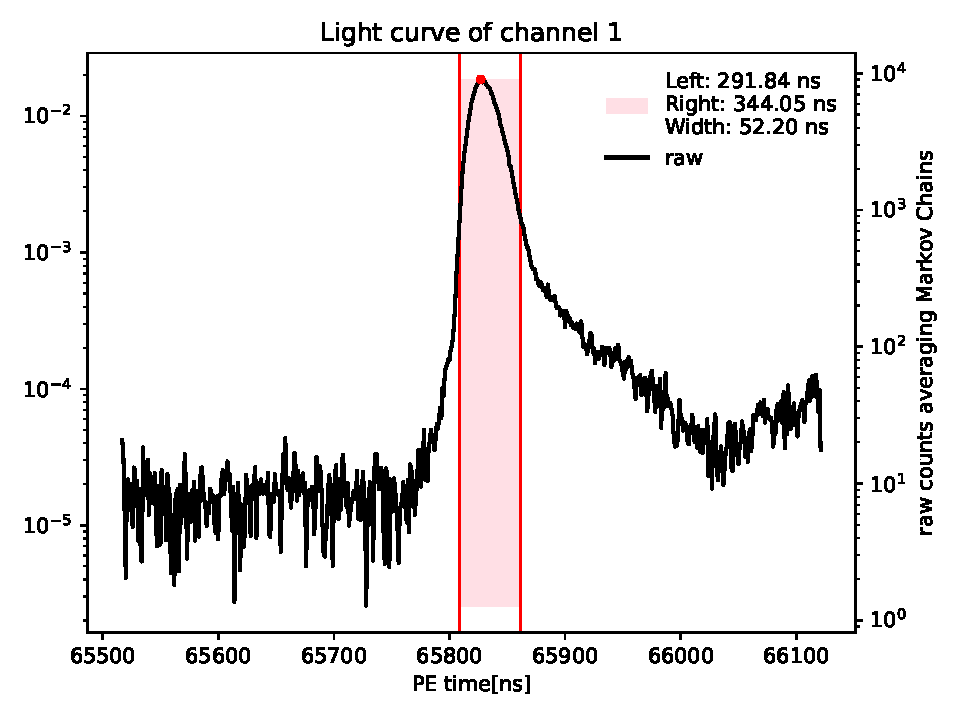
\includegraphics[width=.8\linewidth]{select.pdf}
    \caption*{在 PMT ID 为 1 的通道中,观测到了光变曲线末端具有部分峰的上升结构。红色区间为 10\% 上升下降沿筛选电荷的区间。}
    \caption{单通道的光变曲线与时间窗选择示例}
    \label{fig:selection}
\end{figure}

~\ref{sec:osiris} 节与图~\ref{fig:pulses} 分别提出了多种脉冲展宽的因素,包括激光脉冲的展宽、在 MCP 表面反射或倍增的电子的滞后脉冲
与离子反馈在 MCP 中的反向迁移形成的延迟脉冲,另外也存在激光在其他 PMT 玻璃表面反射至目标 PMT 的可能,分析如下:
\begin{itemize}
    \item 激光脉冲展宽 80 ps,对应电子的延迟应远小于 200 ns;
    \item 被电离的气体分子在 PMT 高压下漂移速度 $\sim10$ m/s,200 ns 对应漂移距离 $\sim2$ μm,而 MCP 的总厚度 $\sim480$ μm;
    \item 液体闪烁体中光速 $\sim2\times10^{8}$ m/s,200 ns 对应 $\sim40$m。
\end{itemize}

综上可知,在 OSIRIS 灵敏体积下,光变曲线中主峰后 200 ns 出现的上升沿主要原因可能是离子反馈,而反射光的影响将在主峰后 200 ns 内。
10\% 的上升下降时间窗筛选具有的优势包括:
\begin{itemize}
    \item 减少图~\ref{fig:pulses} 中前脉冲成分,从而在电荷谱上减少未正确放大的指数项计数;
    \item 减少~\ref{sec:spe-charge} 节中未考虑的离子反馈电荷成分计数;
    \item 对其他光路入射的光子产生的光电子电荷计数有一定抑制作用。
\end{itemize}

\subsection{刻度结果}
\subsubsection{带光强增益刻度}
由图~\ref{fig:variouspe} 可见,在 4 倍主峰后电荷长尾区域双光电子的贡献已经超越了单光电子的贡献,
如果没有使用带光强的拟合方法得到的参数将可能偏离物理真值。
\begin{figure}
    \centering
    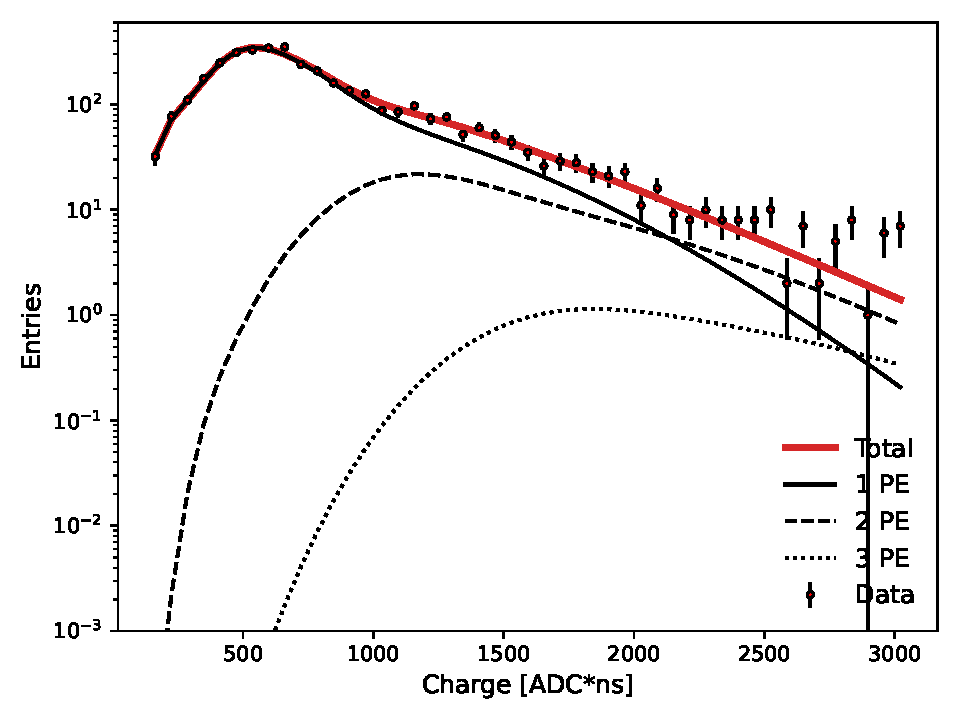
\includegraphics[width=.8\linewidth]{variouspe.pdf}
    \caption{$\mu\sim0.2$ 多光电子拟合实际电荷谱的成分占比}
    \label{fig:variouspe}
\end{figure}

\subsubsection{模型参数}
拟合优度检验得到了良好的结果。
\begin{figure}
    \centering
    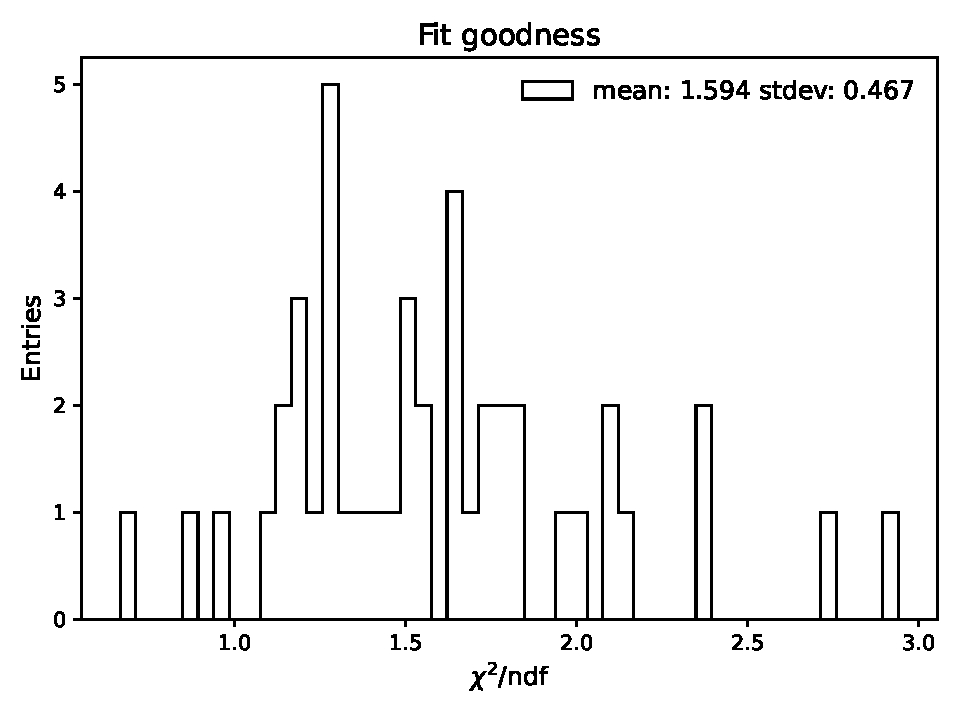
\includegraphics[width=.65\linewidth]{update_chi_sq.pdf}
    \caption{$\chi^2/\text{ndf}$ 分布}
\end{figure}

在~\ref{sec:spe-charge} 节中提出了描述 MCP-PMT 的新参数 $p_0,\lambda$,
在实际刻度中得到两个物理参数的独立分布与二维联合分布。
\begin{figure}
    \centering
    \subcaptionbox{$p_0$ 分布}
      {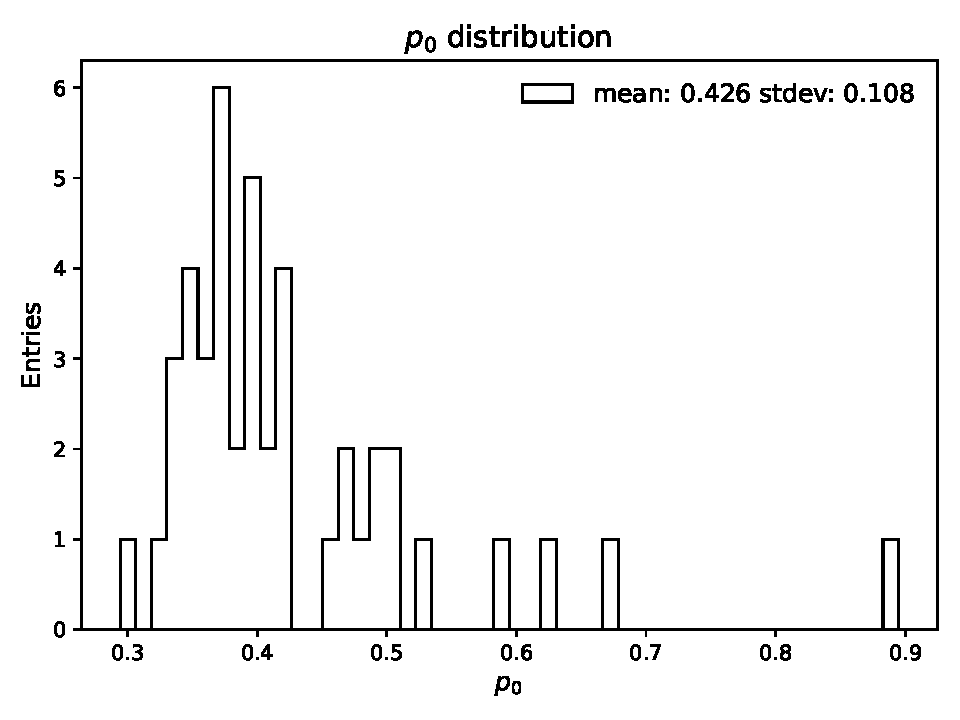
\includegraphics[width=0.48\linewidth]{update_p0.pdf}}
    \subcaptionbox{$\lambda$ 分布}
      {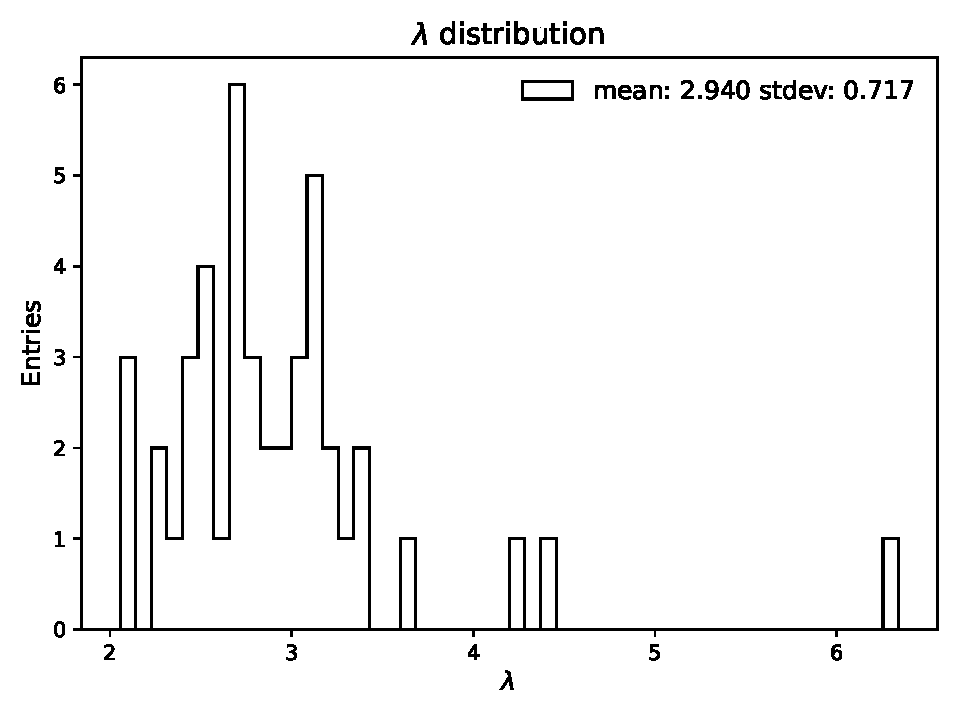
\includegraphics[width=0.48\linewidth]{update_lambda.pdf}}
    \caption{激光刻度参数一维分布}
\end{figure}

\begin{figure}
    \centering
    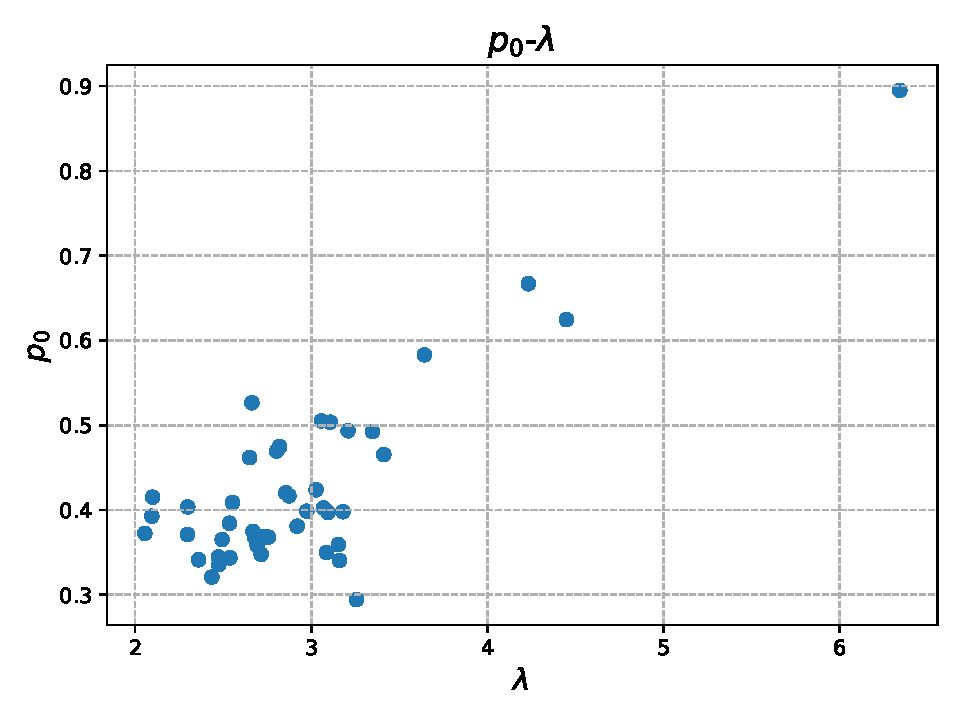
\includegraphics[width=.65\linewidth]{update_p0-lambda.pdf}
    \caption{激光刻度参数二维分布}
\end{figure}

以上结果证明了 20 寸 MCP-PMT 具有与 8 寸相似的行为,且电荷响应能够被 Gamma-Tweedie 混合模型良好地描述。

\subsubsection{分辨率比较}
选取前十支 MCP-PMT 与中国科学院高能物理研究所给出的分辨率做对比,发现使用 Gamma-Tweedie 混合模型得到的分辨率普遍较优。
\begin{figure}
    \centering
    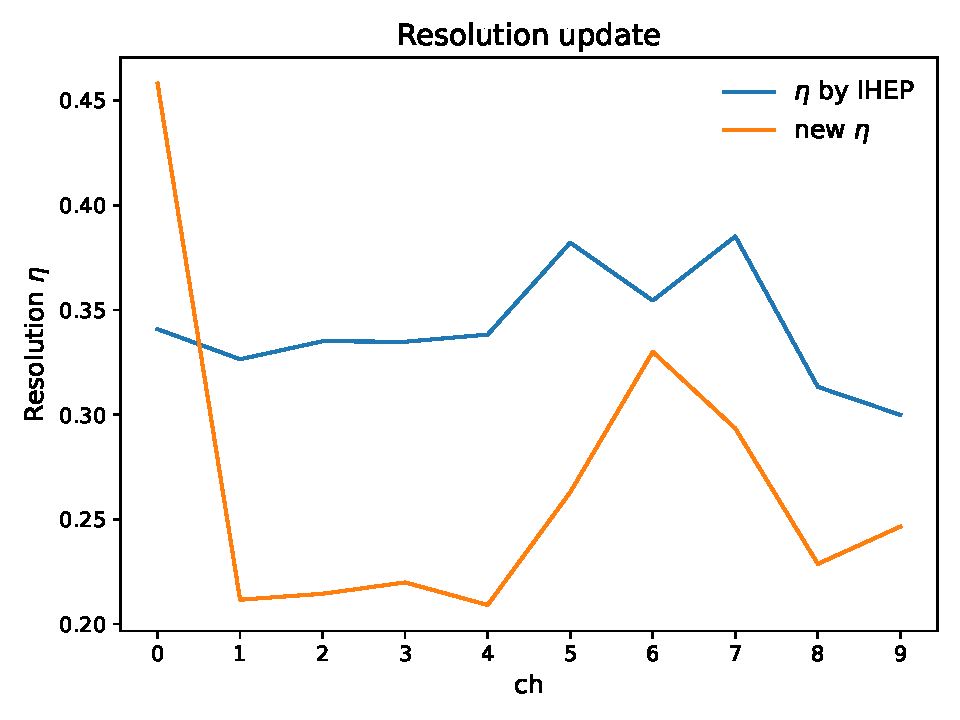
\includegraphics[width=.65\linewidth]{res.pdf}
    \caption{分辨率 $\eta$ 对比}
\end{figure}

\subsection{电荷模型多高斯分解:EM 算法}\label{sec:em}
如~\ref{sec:fsmp} 所述,FSMP 波形分析方法的电荷模型假设为多高斯混合模型。
基于~\ref{sec:spe-charge} 节中所述 Gamma-Tweedie 混合电荷模型,仍需要找到使用若干个高斯分布线性之和尽可能近似该分布的方法,
才能够将第一轮刻度结果作为 FSMP 中采样电荷的依据,进行第二轮波形分析与刻度。

为了找到使用 $m\in\mathbb{N}^{+}$ 个高斯分布近似 Gamma-Tweedie 混合电荷模型的最优解,
首先使用刻度得到的 Gamma-Tweedie 混合模型采样总样本数 $M$ 足够多的随机变量观测集 $\boldsymbol{x}=\{x_1\},\ 1\in{1, 2, \ldots, M}$,
并使用 Expectation Maximization(EM)算法得到极大似然的一组高斯分布线性组合解:
\begin{equation}
    g_{\boldsymbol{\theta}}(x)=\sum_{j=1}^m\lambda_j\mathbf{N}(x;\mu_j, \sigma_j^2),\quad\sum_{j=1}^{m}\lambda_j=1.
\end{equation}

给出参数集 $\boldsymbol{\theta}=(\{\lambda_{j}\},\{\mu_j\},\{\sigma_j^2\})$,
还仍需要隐变量集 $\boldsymbol{Z}=\{Z_{ij}\}$ 表示样本 $x_i$ 是否来自第 $j$ 个高斯分布 $\mathbf{N}_j$:
\begin{equation}
    Z_{ij}=
    \begin{cases}
    1,\quad\text{若}\ x_i\ \text{来自}\ \mathbf{N}_j \\
    0,\quad\text{其他}
    \end{cases}
\end{equation}

至此可以写出似然函数:
\begin{equation}
    \label{eq:log-likelihood}
    \ell(\boldsymbol{\theta};\mathbf{x},\mathbf{Z})=
    \sum_{i=1}^n\sum_{j=1}^mZ_{ij}\log\left(\lambda_j\mathbf{N}(x_i;\mu_j, \sigma_j^2)\right).
\end{equation}

实验中只能观测到样本集 $\boldsymbol{x}$,隐变量 $\boldsymbol{Z}$ 未知,
因此只能极大化~\eqref{eq:log-likelihood} 的期望,即 E-step。

\subsubsection{E-step}
在第 $t$ 步中,在已知 $\boldsymbol{\theta}$ 时的后验概率用 $p_{ij}$ 表示:
\begin{equation}
    p_{ij}^{(t)}=\mathbb{P}_{\boldsymbol{\theta}^{(t)}}\left(Z_{ij}=1
    \mid X_i=x_i\right)=\frac{\lambda_j^{(t)}f(x_i;\mathbf{N}(x;\mu_j^{(t)}, {\sigma_j^2}^{(t)}))}
    {\sum_{r=1}^m\lambda_r^{(t)}f(x_i;\mathbf{N}(x;\mu_j^{(t)}, {\sigma_j^2}^{(t)}))}.
\end{equation}

对数似然函数~\eqref{eq:log-likelihood} 的期望可得:
\begin{equation}
    \label{eq:em_expectation}
    Q(\boldsymbol{\theta}|\boldsymbol{\theta}^{(t)})=
    \mathbb{E}_{\boldsymbol{\theta}^{(t)}}\left[\ell(\boldsymbol{\theta};
    \mathbf{x},\mathbf{Z})\right]=
    \sum_{i=1}^n\sum_{j=1}^mp_{ij}^{(t)}\log\left(\lambda_jf(x_i;\mathbf{N}(x;\mu_j, \sigma_j^2))\right).
\end{equation}

\subsubsection{M-step}\label{sec:m-step}
~\eqref{eq:em_expectation} 化简为:
\begin{equation}
    \begin{aligned}
        Q(\boldsymbol{\theta}|\boldsymbol{\theta}^{(t)})
        &=\sum_{i=1}^n\sum_{j=1}^mp_{ij}^{(t)}\log\left(\lambda_jf(x_i;\mathbf{N}
        (x;\mu_j, \sigma_j^2))\right)\\
        &=\sum_{i=1}^n\sum_{j=1}^mp_{ij}^{(t)}\log\left(
        \lambda_{j}\frac{1}{\sqrt{2\pi}\sigma_j}e^{-\frac{(x_i-\mu_{j})^2}{2\sigma_j^2}}\right)\\
        &\rightarrow\sum_{i=1}^n\sum_{j=1}^mp_{ij}^{(t)}\left(
        {-\frac{(x_i-\mu_{j})^2}{2\sigma_j^2}}-\log{\sigma_j}+\log{\lambda_j}\right)\\
        &\rightarrow-\sum_{i=1}^n\sum_{j=1}^mp_{ij}^{(t)}\left(
        {\frac{(x_i-\mu_{j})^2}{2\sigma_j^2}}+\log{\sigma_j}\right)
        +\sum_{i=1}^n\sum_{j=1}^mp_{ij}^{(t)}\cdot\log{\lambda_j}
    \end{aligned}
\end{equation}

要极大 $Q(\boldsymbol{\theta}|\boldsymbol{\theta}^{(t)})$ ,应有:
\begin{equation}
    \boldsymbol{\theta}^{(t+1)}=\operatorname{argmax}_{\boldsymbol{\theta}}Q(\boldsymbol{\theta}|\boldsymbol{\theta}^{(t)}).
\end{equation}

注意到各高斯参数彼此无约束,显然有更新:
\begin{equation}
    \label{eq:update-lambda}
    \lambda_j^{(t+1)}=\frac1n\sum_{i=1}^np_{ij}^{(t)}.
\end{equation}

$\mu_j,\sigma_j^2$ 参数的更新需要
$\frac{\partial Q(\boldsymbol{\theta}|\boldsymbol{\theta}^{(t)})}{\partial \mu_j}, 
\frac{\partial Q(\boldsymbol{\theta}|\boldsymbol{\theta}^{(t)})}{\partial \sigma_j} = 0$:
\begin{equation}
    \label{eq:freeq}
    \begin{cases}
        \frac{\partial Q(\boldsymbol{\theta}|\boldsymbol{\theta}^{(t)})}{\partial \mu_j}
        =\sum_{i=1}^n\sum_{j=1}^mp_{ij}^{(t)}\cdot\left(\frac{x_i-\mu_j}{\sigma_j}\right) \\
        \frac{\partial Q(\boldsymbol{\theta}|\boldsymbol{\theta}^{(t)})}{\partial \sigma_j}
        =\sum_{i=1}^n\sum_{j=1}^mp_{ij}^{(t)}\cdot\left(-\frac{1}{\sigma_j}+
        \frac{(x_i-\mu_j)^2}{\sigma_j^3}\right)
    \end{cases}
\end{equation}

解~\ref{eq:freeq} 得到更新的参数:
\begin{equation}
    \label{eq:update-theta}
    \begin{cases}
        \mu_j=\frac{\sum_{i=1}^np_{ij}^{(t)}\cdot x_i}{\sum_{i=1}^np_{ij}^{(t)}} \\
        \sigma_j^2=\frac{\sum_{i=1}^np_{ij}^{(t)}\cdot\left(x_i-\mu_j^{(t)}\right)^2}{\sum_{i=1}^np_{ij}^{(t)}}
    \end{cases}
\end{equation}

至此~\eqref{eq:update-lambda} 与~\eqref{eq:update-theta} 构成了完成的 $t\rightarrow t+1$ 步的完整参数更新。
EM 算法收敛至极大似然解的稳定性已经得到了充分的论证。
EM 算法在存在隐变量的问题中是最优秀的算法之一,主要原因包括:
\begin{itemize}
    \item~\eqref{eq:update-lambda} 基于贝叶斯公式,得到的后验概率天然具有非负归一性质;
    \item~\eqref{eq:update-theta} 能确保期望与方差非负,参数更新具有良好的约束。
\end{itemize}

\subsubsection{EM 加速:KMeans 算法初值优化}
在实际使用中,EM 算法的收敛速度饱受诟病。为了加速 EM 算法的收敛,可以提供更接近收敛解的初值。
同时由于 EM 算法只能保证收敛到局域极值而不一定能够收敛到全局极值,本节中将兼顾该问题给出借助 KMeans 算法提供多个初始组的方法:

\begin{enumerate}
    \item 从观测集中随机选出 $m$ 个样本;
    \item 将与样本 $k$ 距离最小的样本归类为第 $k$ 个聚类;
    \item 对第 $k$ 个聚类的所有样本取平均,作为聚类 $k$ 的新均值(中心);
    \item 重复 2-3 直至给定步数或均值收敛;
    \item 计算每个聚类中样本点至聚类中心的距离均方作为该聚类方差。
\end{enumerate}

对于一维至三维数据,距离容易定义,KMeans 是较为简单有效的分聚类算法,适合作为 EM 算法的初值。

\subsubsection{EM 加速:向量 Aitken 加速的 Steffenson 形式}
向量 Aitken 是一种得到广泛应用的加速收敛的方法。它基于原序列 $\boldsymbol{\phi}^{(t)}$ 提出收敛更快的序列:
\begin{equation}
    \label{eq:vector-aitken}
    \boldsymbol{\phi}_{VA}^{(1)}=\boldsymbol{\phi}^{(0)}-
    \frac{||\boldsymbol{\phi}^{(1)}-\boldsymbol{\phi}^{(0)}||^2
    (\boldsymbol{\phi}^{(0)}-2\boldsymbol{\phi}^{(1)}+\boldsymbol{\phi}^{(2)})}
    {||\boldsymbol{\phi}^{(0)}-2\boldsymbol{\phi}^{(1)}+\boldsymbol{\phi}^{(2)}||^2}.
\end{equation}

Steffenson 方式是一种不动点迭代的方法,将~\ref{sec:m-step} 中定义的参数更新步骤记为 $M(\cdot)$,由于 $\boldsymbol{\phi}$ 有确定的收敛值 $\boldsymbol{\phi}^*$
序列更新 $\boldsymbol{\phi}\rightarrow M(\boldsymbol{\phi})\rightarrow\cdots\rightarrow\boldsymbol{\phi}^{*}$ 可以视为趋近不动点 $\boldsymbol{\phi}^*$ 的迭代行为,
应用于~\eqref{eq:vector-aitken} 即得向量 Aitken 的 Steffen 形式:
\begin{equation}
    \label{eq:steffenson}
    \phi_{VA}^{(2)}=\phi_{VA}^{(1)}-\frac{||M(\phi_{VA}^{(1)})-
    \phi_{VA}^{(1)}||^2(\phi_{VA}^{(1)}-2M(\phi_{VA}^{(1)})+M^{(2)}
    (\phi_{VA}^{(1)}))}{||\phi_{VA}^{(1)}-2M(\phi_{VA}^{(1)})+M^{(2)}(\phi_{VA}^{(1)})||^2}.
\end{equation}

考虑到~\eqref{eq:vector-aitken} 与~\eqref{eq:steffenson} 并不像原始的 EM 算法,不能保证参数更新的合法性,
因此在本研究中 EM 算法的加速调整如下:
\begin{enumerate}
    \item[1.] 利用 $M(\cdot)$ 由 $\boldsymbol{\theta}^{(0)}$ 得到 $\boldsymbol{\theta}^{(1)}, \boldsymbol{\theta}^{(2)}$;
    \item[2.] 利用~\eqref{eq:vector-aitken} 只更新 $\boldsymbol{\phi}_{VA}^{(1)}$;
    \item[3.] 判断 $\boldsymbol{\phi}_{VA}^{(1)}$ 合法性(是否非负):
    \begin{enumerate}
        \item[3.1 ] 若合法,以 $\mu$ 升序重排,~\eqref{eq:update-lambda} 计算 $(\lambda^{(0)}, \boldsymbol{\phi}_{VA}^{(1)})$ 下的 $\lambda^{(1)}$,
        初始参数 $\boldsymbol{\theta}_{VA}^{(1)}=(\lambda^{(1)}, \boldsymbol{\phi}_{VA}^{(1)})$ 重复 1-3;
        \item[3.2 ] 若非法,利用 $M(\cdot)$ 更新初始参数 $\boldsymbol{\theta}^{(1)},\boldsymbol{\theta}^{(2)}, \boldsymbol{\theta}^{(3)}$ 重复 2-3;
    \end{enumerate}
    \item[4.] 直至 $||\theta_{VA}^{(t+1)}-\theta_{VA}^{(t)}||^2\leq\delta$ 结束迭代。
\end{enumerate}

\subsection{电荷模型多高斯分解结果}

为了决定使用高斯的数量以及近似的准确度,选取贝叶斯信息准则(Bayesian information criterion,以下简称 BIC):
\begin{equation}
    \label{eq:bic}
    \text{BIC}=k\ln{n}-2\ell
\end{equation}

其中 $k$ 为模型自由度,$n$ 为样本数,$\ell$ 为对数似然函数。
BIC 用于在有限模型中进行模型选择,与~\ref{sec:criterion} 中使用的 $\chi^2/\text{ndf}$ 相比更倾向于比较不同模型间的优劣,
且使用对数似然函数,与 EM 算法契合。BIC 最小的模型在模型集中最优\cite{10.1214/aos/1176344136}。

~\eqref{eq:bic} 使用系数 $k$ 使得对模型自由度有与样本数 $n$ 呈对数的惩罚关系,因此能够有效减少过拟合情形的发生。
对于确定高斯分布的个数,BIC 是合适的选择。

本研究中使用随机数种子 123,使用刻度的分布采样 10000 个随机数并使用~\ref{sec:em} 节中所述的方法进行分解,
并比较 BIC。本研究对刻度参数集使用 3 至 6 个高斯分布,观察到对于大多数参数集 4 个高斯与 5 个高斯 BIC 接近且优于其他个数,
但对于少数情况会出现 5 个高斯在主峰前由单个二次倍增峰贡献处近似较 4 个高斯优的情况,如图~\ref{fig:multi-image} 所示,
其中 $\text{BIC}_4=140560.1>\text{BIC}_5=140420.4$。

\begin{figure}
    \centering
    \subcaptionbox{4 个高斯分解}
      {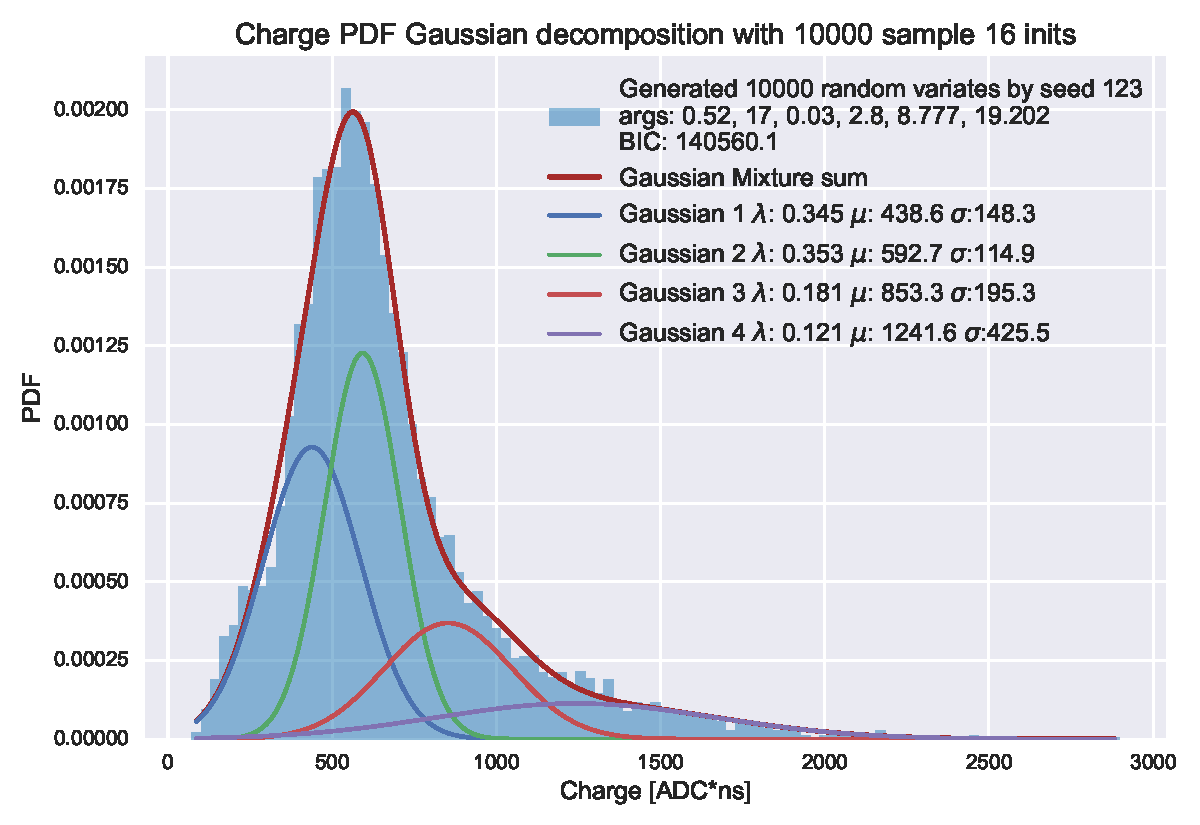
\includegraphics[width=0.48\linewidth]{GMM_4-13.pdf}}
    \subcaptionbox{5 个高斯分解}
      {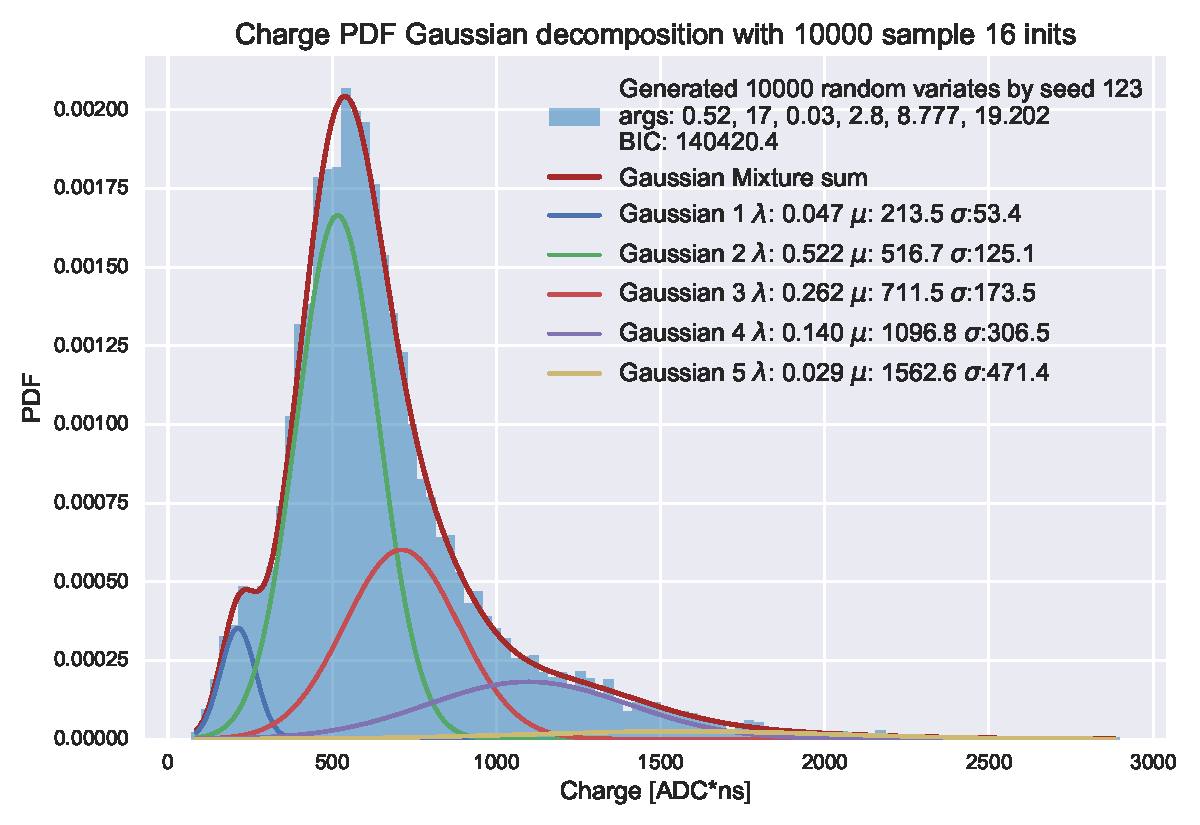
\includegraphics[width=0.48\linewidth]{GMM_5-13.pdf}}
    \caption{利用 BIC 判断 4 个与 5 个高斯分解的优劣}
    \label{fig:multi-image}
\end{figure}

可以得出结论:5 个高斯分解对于主峰前单个二次倍增峰(即 Tweedie 成分)描述较 4 个高斯分解略优,较其他个数优。

\subsection{迭代结果对比}
由使用 JWAPtool 粗筛得到的结果与第一轮刻度结果对比:
\begin{figure}
    \centering
    \subcaptionbox{增益 $\mu$ 对比}
      {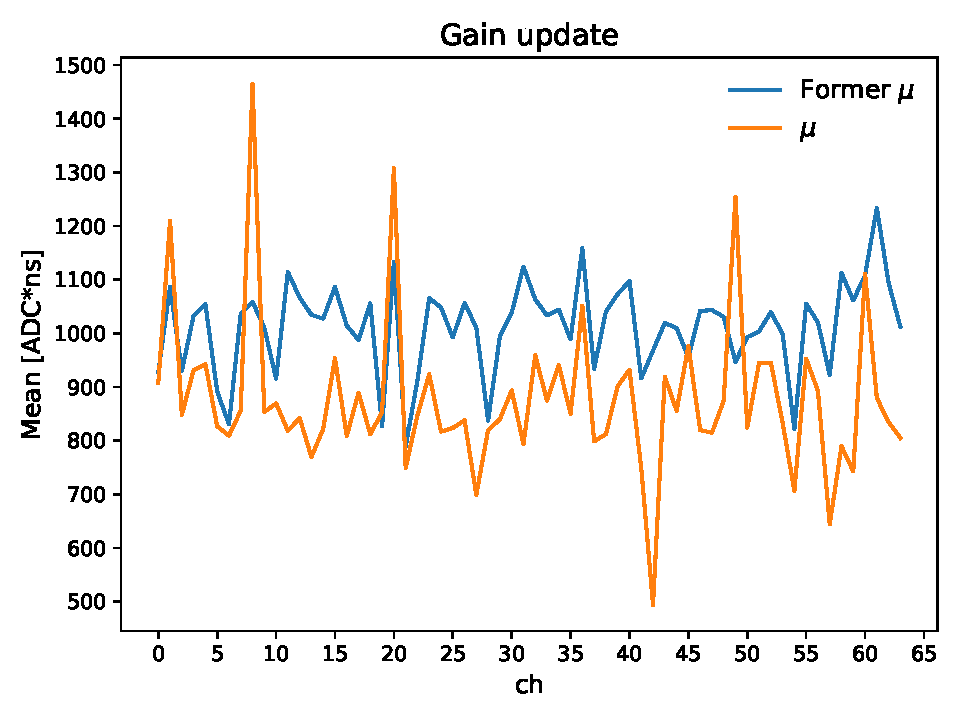
\includegraphics[width=0.48\linewidth]{gain.pdf}}
    \subcaptionbox{分辨率 $\eta$ 对比}
      {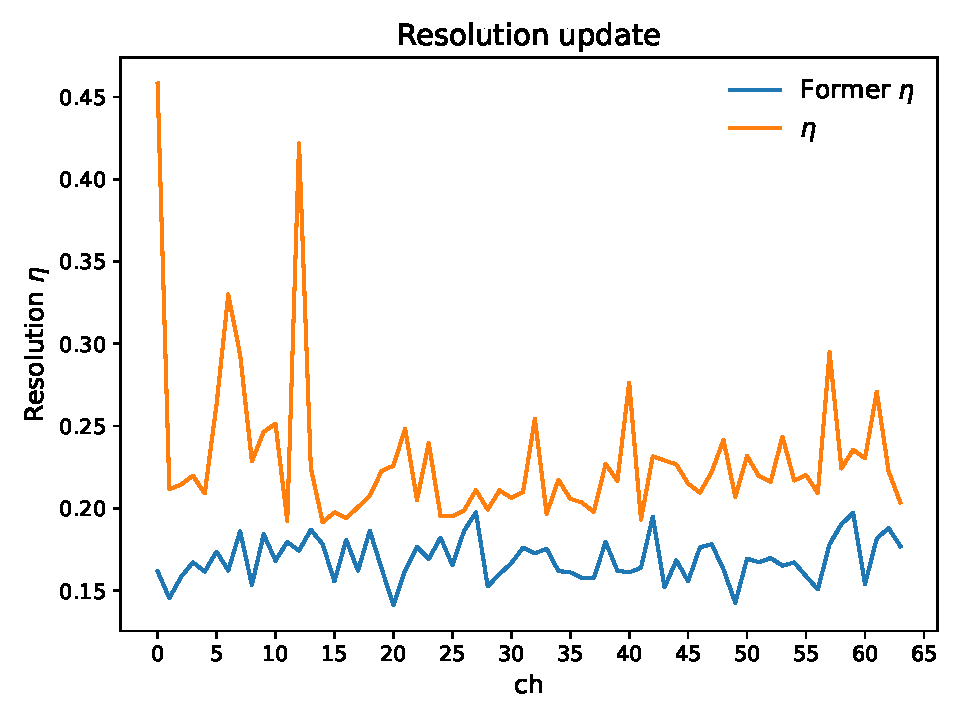
\includegraphics[width=0.48\linewidth]{resolution.pdf}}
    \caption{迭代结果对比}
\end{figure}

本研究将继续迭代至前后的物理结果收敛,并认为收敛值为拟合得到的 PMT 最终刻度结果。

% !TeX root = ../thuthesis-example.tex

\chapter{结果}

\section{工作总结}
本论文将 8 寸 MCP-PMT 的电荷模型应用在 JUNO 等中微子探测实验广泛应用的 20 寸 MCP-PMT 上,
证实该电荷模型具有较好的适用性。

为了提高电荷长尾拟合的准确率以及赋予拟合方法在高光强工作条件下的适用性,论文推导得到了任意光电子数目的电荷谱响应,
基于傅里叶变换变换得到了能够适应不同光强的拟合方法,除了提高激光数据增益刻度的准确性,
也为该 MCP-PMT 在高光强场景下的应用提供了理论无偏的拟合工具。

论文基于 FSMP 波形分析方法得到电荷谱,并找到了由电荷模型近似极大似然高斯混合模型解的方法,
在 OSIRIS 探测器上实现了各 MCP-PMT 的增益刻度与高斯混合电荷模型近似,
使得波形分析方法迭代成为现实。

\section{问题与改进方向}
论文还需要进行多轮迭代,直到达到参数收敛的标准。

论文基于 FSMP 波形分析方法得到了光电子到达时间的归一化曲线,即光变曲线,
能够以此进行单光电子波形的重新筛选以得到更准确的波形分析结果。
以后的工作将着力于实现该想法。



% 其他部分
\backmatter

% 参考文献
\bibliography{ref/refs}  % 参考文献使用 BibTeX 编译
% \printbibliography       % 参考文献使用 BibLaTeX 编译

% 附录
% 本科生需要将附录放到声明之后,个人简历之前
\appendix
% % !TeX root = ../thuthesis-example.tex

\begin{survey}
\label{cha:survey}

\title{Title of the Survey}
\maketitle


\tableofcontents


本科生的外文资料调研阅读报告。


\section{Figures and Tables}

\subsection{Figures}

An example figure in appendix (Figure~\ref{fig:appendix-survey-figure}).

\begin{figure}
  \centering
  \includegraphics[width=0.6\linewidth]{example-image-a.pdf}
  \caption{Example figure in appendix}
  \label{fig:appendix-survey-figure}
\end{figure}


\subsection{Tables}

An example table in appendix (Table~\ref{tab:appendix-survey-table}).

\begin{table}
  \centering
  \caption{Example table in appendix}
  \begin{tabular}{ll}
    \toprule
    File name       & Description                                         \\
    \midrule
    thuthesis.dtx   & The source file including documentation and comments \\
    thuthesis.cls   & The template file                                   \\
    thuthesis-*.bst & BibTeX styles                                       \\
    thuthesis-*.bbx & BibLaTeX styles for bibliographies                  \\
    thuthesis-*.cbx & BibLaTeX styles for citations                       \\
    \bottomrule
  \end{tabular}
  \label{tab:appendix-survey-table}
\end{table}


\section{Equations}

An example equation in appendix (Equation~\eqref{eq:appendix-survey-equation}).
\begin{equation}
  \frac{1}{2 \uppi \symup{i}} \int_\gamma f = \sum_{k=1}^m n(\gamma; a_k) \mathscr{R}(f; a_k)
  \label{eq:appendix-survey-equation}
\end{equation}


\section{Citations}

Example\cite{dupont1974bone} citations\cite{merkt1995rotational} in appendix
\cite{dupont1974bone,merkt1995rotational}.


% 默认使用正文的参考文献样式;
% 如果使用 BibTeX,可以切换为其他兼容 natbib 的 BibTeX 样式。
\bibliographystyle{unsrtnat}
% \bibliographystyle{IEEEtranN}

% 默认使用正文的参考文献 .bib 数据库;
% 如果使用 BibTeX,可以改为指定数据库,如 \bibliography{ref/refs}。
\printbibliography

\end{survey}
       % 本科生:外文资料的调研阅读报告
% % !TeX root = ../thuthesis-example.tex

\begin{translation}
\label{cha:translation}

\title{书面翻译题目}
\maketitle

\tableofcontents


本科生的外文资料书面翻译。


\section{图表示例}

\subsection{图}

附录中的图片示例(图~\ref{fig:appendix-translation-figure})。

\begin{figure}
  \centering
  \includegraphics[width=0.6\linewidth]{example-image-a.pdf}
  \caption{附录中的图片示例}
  \label{fig:appendix-translation-figure}
\end{figure}


\subsection{表格}

附录中的表格示例(表~\ref{tab:appendix-translation-table})。

\begin{table}
  \centering
  \caption{附录中的表格示例}
  \begin{tabular}{ll}
    \toprule
    文件名          & 描述                         \\
    \midrule
    thuthesis.dtx   & 模板的源文件,包括文档和注释 \\
    thuthesis.cls   & 模板文件                     \\
    thuthesis-*.bst & BibTeX 参考文献表样式文件    \\
    thuthesis-*.bbx & BibLaTeX 参考文献表样式文件  \\
    thuthesis-*.cbx & BibLaTeX 引用样式文件        \\
    \bottomrule
  \end{tabular}
  \label{tab:appendix-translation-table}
\end{table}


\section{数学公式}

附录中的数学公式示例(公式\eqref{eq:appendix-translation-equation})。
\begin{equation}
  \frac{1}{2 \uppi \symup{i}} \int_\gamma f = \sum_{k=1}^m n(\gamma; a_k) \mathscr{R}(f; a_k)
  \label{eq:appendix-translation-equation}
\end{equation}


\section{文献引用}

附录\cite{dupont1974bone}中的参考文献引用\cite{merkt1995rotational}示例
\cite{dupont1974bone,merkt1995rotational}。


\appendix

\section{附录}

附录的内容。


% 书面翻译的参考文献
% 默认使用正文的参考文献样式;
% 如果使用 BibTeX,可以切换为其他兼容 natbib 的 BibTeX 样式。
\bibliographystyle{unsrtnat}
% \bibliographystyle{IEEEtranN}

% 默认使用正文的参考文献 .bib 数据库;
% 如果使用 BibTeX,可以改为指定数据库,如 \bibliography{ref/refs}。
\printbibliography

% 书面翻译对应的原文索引
\begin{translation-index}
  \nocite{mellinger1996laser}
  \nocite{bixon1996dynamics}
  \nocite{carlson1981two}
  \bibliographystyle{unsrtnat}
  \printbibliography
\end{translation-index}

\end{translation}
  % 本科生:外文资料的书面翻译
% !TeX root = ../thuthesis-example.tex

\chapter{补充内容}

附录是与论文内容密切相关、但编入正文又影响整篇论文编排的条理和逻辑性的资料,例如某些重要的数据表格、计算程序、统计表等,是论文主体的补充内容,可根据需要设置。

附录中的图、表、数学表达式、参考文献等另行编序号,与正文分开,一律用阿拉伯数字编码,
但在数码前冠以附录的序号,例如“图~\ref{fig:appendix-figure}”,
“表~\ref{tab:appendix-table}”,“式\eqref{eq:appendix-equation}”等。


\section{插图}

% 附录中的插图示例(图~\ref{fig:appendix-figure})。

\begin{figure}
  \centering
  \includegraphics[width=0.6\linewidth]{example-image-a.pdf}
  \caption{附录中的图片示例}
  \label{fig:appendix-figure}
\end{figure}


\section{表格}

% 附录中的表格示例(表~\ref{tab:appendix-table})。

\begin{table}
  \centering
  \caption{附录中的表格示例}
  \begin{tabular}{ll}
    \toprule
    文件名          & 描述                         \\
    \midrule
    thuthesis.dtx   & 模板的源文件,包括文档和注释 \\
    thuthesis.cls   & 模板文件                     \\
    thuthesis-*.bst & BibTeX 参考文献表样式文件    \\
    thuthesis-*.bbx & BibLaTeX 参考文献表样式文件  \\
    thuthesis-*.cbx & BibLaTeX 引用样式文件        \\
    \bottomrule
  \end{tabular}
  \label{tab:appendix-table}
\end{table}


\section{数学表达式}

% 附录中的数学表达式示例(式\eqref{eq:appendix-equation})。
\begin{equation}
  \frac{1}{2 \uppi \symup{i}} \int_\gamma f = \sum_{k=1}^m n(\gamma; a_k) \mathscr{R}(f; a_k)
  \label{eq:appendix-equation}
\end{equation}


\section{文献引用}

附录\cite{dupont1974bone}中的参考文献引用\cite{zhengkaiqing1987}示例
\cite{dupont1974bone,zhengkaiqing1987}。

\printbibliography


% 致谢
% !TeX root = ../thuthesis-example.tex

\begin{acknowledgements}
  衷心感谢导师×××教授和物理系××副教授对本人的精心指导。他们的言传身教将使我终生受益。

  在美国麻省理工学院化学系进行九个月的合作研究期间,承蒙 Robert Field 教授热心指导与帮助,不胜感激。

  感谢×××××实验室主任×××教授,以及实验室全体老师和同窗们学的热情帮助和支持!

  本课题承蒙国家自然科学基金资助,特此致谢。
\end{acknowledgements}


% 声明
% 本科生开题报告不需要
\statement
% 将签字扫描后的声明文件 scan-statement.pdf 替换原始页面
% \statement[file=scan-statement.pdf]
% 本科生编译生成的声明页默认不加页脚,插入扫描版时再补上;
% 研究生编译生成时有页眉页脚,插入扫描版时不再重复。
% 也可以手动控制是否加页眉页脚
% \statement[page-style=empty]
% \statement[file=scan-statement.pdf, page-style=plain]

% 个人简历、在学期间完成的相关学术成果
% 本科生可以附个人简历,也可以不附个人简历
% !TeX root = ../thuthesis-example.tex

\begin{resume}

  \section*{个人简历}

  2002 年 03 月 17 日出生于浙江省宁波市。

  2020 年 9 月考入清华大学未央书院数理基础科学+工程物理专业。

  \section*{在学期间完成的相关学术成果}

  \subsection*{学术报告}

  2023 年 2 月于第 23 次 JUNO 合作组会线下汇报 MCP-PMT 刻度情况。

\end{resume}


% 指导教师/指导小组评语
% 本科生不需要
% % !TeX root = ../thuthesis-example.tex

\begin{comments}
% \begin{comments}[name = {指导小组评语}]
% \begin{comments}[name = {Comments from Thesis Supervisor}]
% \begin{comments}[name = {Comments from Thesis Supervision Committee}]

  论文提出了……

\end{comments}


% 答辩委员会决议书
% 本科生不需要
% % !TeX root = ../thuthesis-example.tex

\begin{resolution}

  论文提出了……

  论文取得的主要创新性成果包括:

  1. ……

  2. ……

  3. ……

  论文工作表明作者在×××××具有×××××知识,具有××××能力,论文××××,答辩××××。

  答辩委员会表决,(×票/一致)同意通过论文答辩,并建议授予×××(姓名)×××(门类)学博士/硕士学位。

\end{resolution}


% 本科生的综合论文训练记录表(扫描版)
% \record{file=scan-record.pdf}

\end{document}
